% \begin{filecontents*}{\jobname.xmpdata}
%   \Title{Pro gradu -tutkielma}
%   \Author{Ewert Kupiainen}
% \end{filecontents*}

\documentclass[a4paper,12pt,twoside]{article}
\usepackage[finnish]{babel}
\usepackage[T1]{fontenc}
\usepackage[utf8]{inputenc}
\usepackage{amsthm}
\usepackage{amsmath}
\usepackage{amsfonts}
\usepackage{amssymb}
\usepackage{graphicx}
\usepackage{iftex}
\ifPDFTeX
\usepackage[tagpdf]{axessibility}
\fi
\usepackage[a-3b]{pdfx}
\usepackage[toc, title, header]{appendix}
\usepackage[pdfa]{hyperref}
\usepackage{caption}
\usepackage{lipsum}
\usepackage{listings}
\usepackage{xcolor} % Optional: for color customization
\usepackage{enumitem}
\usepackage{booktabs}
\usepackage{makecell}
\usepackage{tabularx}
\usepackage{cleveref}

\usepackage{etoolbox}
\preto{\section}{\clearpage}
\lstset{
  basicstyle=\ttfamily\small,
  breaklines=true,
  frame=single
}
\usepackage{geometry}
\geometry{
  a4paper,
  total={150mm,237mm},
  left=30mm,
  top=30mm,
}
\lstdefinelanguage{yaml}{
  % Tell listings that underscore is a valid part of a word
  alsoletter={-},
  keywords={true,false,null,y,n},
  keywordstyle=\color{darkgray}\bfseries,
  comment=[l]{\#},
  commentstyle=\color{gray}\ttfamily,
  stringstyle=\color{teal}\ttfamily,
  morestring=[b]',
  morestring=[b]",
  % Add both identifiers here
  keywords=[2]{name, description, tables, base_table, database, schema, table,
    dimensions, expr, data_type, facts, access_modifier, metrics,
  primary_key, columns},
  keywordstyle=[2]\color{blue}\bfseries,
}
\renewcommand{\Re}{\mathbb{R}}
\renewcommand{\L}{\mathcal{L}}
\newcommand{\T}{\intercal}
\newcommand{\M}[1]{\mathbf{#1}}
\newcommand{\N}{\mathbb{N}}
\newcommand{\tfidf}{\operatorname{tfidf}}
\pagenumbering{roman} %For accessibility

\begin{document}
%Suomenkieliset ympäristöt:

\theoremstyle{plain}
\newtheorem{theorem}{Lause}
\newtheorem{lemma}{Lemma}
\newtheorem{corollary}{Seuraus}
%
\theoremstyle{definition}
\newtheorem{definition}{M\"a\"aritelm\"a}
\newtheorem{example}{Esimerkki}
%
\theoremstyle{remark}
\newtheorem{remark}{Huomautus}

%Määrittele tässä aika, työn, kirjoittajan ja ohjaajien tiedot

\newcommand{\tekija}{{Omar Mayani}} %tekijän nimi
\newcommand{\titteli}{{}} %voi jättää tyhjäksi
\newcommand{\otsikko}{{Joku otsikko}}   %Gradun otsikko
\newcommand{\tutkielma}{{Pro gradu }}   %Pro Gardu tai LuK. Huom kirjoitusasu, välilyönti lopussa graduille
\newcommand{\aika}{{Kesäkuu 2020}}   %Kuukausi ja vuosi
\newcommand{\paaaine}{{Matematiikka}} %tai Tilastotiede
\newcommand{\ohjaaja}{{Prof. Ion Petre}} %Ohjaajan titteli (Prof./Dos./FT) ja nimi
\newcommand{\tarkastaja}{{Markus Ylikojola}} %Toisen tarkastajan titteli (Prof./Dos./FT) ja nimi

\pagenumbering{roman} %Saavuttavuuden takija alussa sivunurot roomalaisittain, tutkielman alusta arabialaisittain.
\pagestyle{empty}  %ei sivunumeroa sivun alareunaan

\begin{center}
  
\includegraphics[width=10cm]{media/UTU_logo_FI.jpg} %talleta kuva linkistä omaan hakemistoosi
\end{center}

\vspace{3.0cm}
\begin{center}\large
  {\sc \otsikko}
\end{center}

\vspace{0.5cm}
\begin{center}
  \titteli \tekija
\end{center}

\vspace{0.5cm}
\begin{center}
  \tutkielma -tutkielma\\
  \aika
\end{center}

\vspace{2.5cm}

\vspace{2.5cm}
\begin{center}
  MATEMATIIKAN JA TILASTOTIETEEN LAITOS
\end{center}

\newpage%\null

\noindent
\begin{tabular}{l}
  {\bf Tarkastajat:}\\
  \ohjaaja \\
  \tarkastaja
\end{tabular}

\vspace{20cm}

%Pakollinen ilmoitus Turnitin-järjestelmän käytöstä:
\noindent Turun yliopiston laatujärjestelmän mukaisesti tämän julkaisun alkuperäisyys on tarkastettu
Turnitin OriginalityCheck-järjestelmällä

\cleardoublepage

\noindent
TURUN YLIOPISTO, Matematiikan ja tilastotieteen laitos\\
\\
\tutkielma -tutkielma \\
{\bf Pääaine:} \paaaine \\
{\bf Tekijä:}  \tekija \\
{\bf Otsikko:} \otsikko \\
{\bf Ohjaaja:} \ohjaaja \\
{\bf Sivumäärä:} xx sivua + liitteet xx sivua \\ %täytä sivumäärät!
{\bf Aika:} \aika \\
\rule{\textwidth}{.2mm}\\
\\

\vspace{4mm}\noindent Kirjoita tähän tiivistelmä. Laita $\backslash${noindent}-komento kappaleen
alkuun, niin \LaTeX\, ei sisennä ensimmäistä riviä.

\vspace{4mm}\noindent Komento $\backslash$vspace taasen jättää sopivan välin kappaleiden väliin - 4mm näyttää aika hyvältä.

\vspace{4mm}\noindent Kirjoita tiivistelmä napakasti ja kaikenlaista toistoa välttäen.

\vspace{4mm}\noindent Asiasanat: tiivistelmäsivu, Pro gradu -tutkielma, \LaTeX-ladontajärjestelmä.

\cleardoublepage

\tableofcontents
%Aja laTeX-käännös uudelleen saadaksesi ajantasaisen sisällysluettelon

\cleardoublepage

\pagestyle{plain}
\pagenumbering{arabic} % Saavutettavuus: Aloitetaan arabialaisilla numeroilla tältä sivulta

\begin{center}
  
\includegraphics[width=10cm]{media/Teknologiateollisuus-logo-musta.png}
\end{center}
Tämän pro gradu -tutkielman tutkimustyötä on tuettu Teknologiateollisuuden 100-vuotissäätiön myöntämällä apurahalla.

% Dense in this paper != dense as in rationals are dense in reals.
% When we say low dimensional, we mean relative to the size of the vocabulary. So a 300-dimensional embedding for a vocabulary of 10,000 words is low dimensional.

\thispagestyle{plain}
\begin{center}
  \large{MERKINTÄTAVOISTA}
\end{center}
Tässä opinnäytetyössä käytetään seuraavia merkintöjä ja termejä.

\begin{align*}
  &\mathbb{R} &&\text{reaalilukujen joukko} \\
  &\mathbb{N} &&\text{luonnollisten lukujen joukko } \{1, 2, 3, \dots\} \\
  &A^{\top} &&\text{matriisin tai vektorin } A \text{ transpoosi} \\
  &\odot &&\text{Hadamard-tulo (alkioittainen kertolasku)} \\
  &[A \,\|\, B] &&\text{vektorien tai matriisien vaakasuuntainen ketjuttaminen} \\
  &|S| &&\text{joukon tai sekvenssin } S \text{ alkioiden lukumäärä} \\
  &\mathbf{1}\{\cdot\} &&\text{indikaattorifunktio} \\
  &\mathcal{V} = \{v_1, \dots, v_{|\mathcal{V}|}\} &&\text{sanasto (kaikkien käytettävien tokenien joukko)} \\
  &w_t \in \mathcal{V} &&\text{korpuksen ajanhetken } t \text{ tokeni} \\
  &\mathcal{W} = (w_1, \dots, w_{|\mathcal{W}|}) &&\text{korpus (havaittu tokenijono)} \\
  &x(v_j) \in \{0, 1\}^{1 \times |\mathcal{V}|} &&\text{tokenin } v_j \text{ one-hot-esitys (rivivektori)} \\
  &e(v_j) \in \mathbb{R}^{1 \times d} &&\text{tokenin } v_j \text{ tiheä upotusvektori (rivivektori)} \\
  &E \in \mathbb{R}^{|\mathcal{V}| \times d} &&\text{tokenien upotusmatriisi} \\
  &H \in \mathbb{R}^{T \times d} &&\text{esitysmatriisi (jonon pituus } T\text{, upotusdimensio } d\text{)} \\
  &\ell \in \mathbb{R}^{1 \times |\mathcal{V}|} &&\text{normalisoimaton pistemäärävektori (logittivektori)} \\
  &J(\theta) &&\text{häviöfunktio} \\
  &\theta &&\text{mallin opittavien parametrien joukko} \\
  &\Delta(\mathcal{V}) &&\text{sanaston } \mathcal{V} \text{ yli määriteltyjen todennäköisyysjakaumien joukko}
\end{align*}

\tableofcontents
\section{Johdanto}

Kielimallit ovat luonnollisen kielen käsittelyn malleja, joiden avulla
voidaan kuvata tekstin tilastollista rakennetta tai tuottaa uutta tekstiä.
Autoregressiivisessa kielimallinnuksessa malli ennustaa seuraavaa sanaa
(tai tokenia eli tekstin käsittely-yksikköä) aiemman kontekstin perusteella
\cite{jurafsky2023speech, bengio2003neural}. Tekstiä voidaan generoida
valitsemalla mallin ennustamasta jakaumasta seuraava token, liittämällä se
kontekstiin ja toistamalla menettelyä päivitetyllä kontekstilla. Tämä periaate yhdistää klassisia
n-gram-malleja \cite{shannon1948mathematical} ja nykyaikaisia transformer pohjaisia kielimalleja \cite{vaswani2017attention}, vaikka niiden
tavat esittää kontekstia ja muodostaa ennustejakauma eroavat huomattavasti.

Kielimallien kehityksessä keskeinen muutos on ollut siirtyminen
diskreeteistä tekstiesityksistä opittuihin jatkuviin esityksiin \cite{mikolov2013efficient} sekä
esiintymismääriin perustuvista malleista neuroverkkopohjaiseen
mallinnukseen \cite{werbos1974beyond, rumelhart1986learning}. Upotusvektoreiden avulla tokenit esitetään vektoriavaruudessa, jossa niiden väliset suhteet voidaan oppia aineistosta. Samalla neuroverkon parametreja optimoidaan tuottamaan opetusaineistoa vastaavia jakaumia. Nykyaikaisissa
dekooderipohjaisissa Transformer-malleissa kontekstin käsittely perustuu
itsehuomioon \cite{vaswani2017attention}, jonka avulla tokenien esityksiä muodostetaan suhteessa
muihin kontekstin tokeneihin. Kielimallien toiminnan ymmärtäminen edellyttää
siten tekstiesitysten, todennäköisyysmallinnuksen, optimoinnin ja
neuroverkkoarkkitehtuurin tarkastelua yhtenä kokonaisuutena.

Suurten kielimallien sovellukset eivät rajoitu vapaamuotoisen tekstin
tuottamiseen. Kielimalleja voidaan liittää järjestelmiin, joissa osa niiden
tuottamista tokeneista tulkitaan työkalukutsuina
\cite{schick2023toolformer, yao2023react}. Tällöin kielimallia ympäröivä
ohjelmisto voi suorittaa laskentaa, tehdä verkkohakuja tai käsitellä
tietokantakyselyitä. Yksi käytännössä merkittävä sovelluskohde on
luonnollisen kielen muuntaminen SQL-kyselyiksi eli Text-to-SQL
\cite{liu2024survey, deng2022recent}. Sen tavoitteena on mahdollistaa
tietokantojen hyödyntäminen ilman, että käyttäjän tarvitsee itse kirjoittaa
SQL-kyselyitä tai tuntea tietokannan rakennetta yksityiskohtaisesti.

Text-to-SQL-järjestelmän hyödyllisyys riippuu kuitenkin siitä, kuinka
luotettavasti se kykenee yhdistämään käyttäjän tiedontarpeen tietokannan
rakenteeseen ja muodostamaan tarkoitusta vastaavan kyselyn
\cite{yu2018spider, li2024bird}. Syntaktisesti kelvollinen SQL-kysely ei
välttämättä vastaa käyttäjän tarkoittamaa kysymystä. Luotettavuuden kannalta
on myös olennaista, säilyykö järjestelmän tulkinta johdonmukaisena saman
kysymyksen toistoissa ja silloin, kun kysymyksen esitystapaa muutetaan
sen merkitystä muuttamatta. Nämä kysymykset motivoivat kielimallipohjaisten
järjestelmien empiiristä arviointia.

Tämän tutkielman tavoitteena on jäsentää autoregressiivisen
kielimallinnuksen matemaattisia perusteita ja tarkastella
kielimallipohjaisen Text-to-SQL-järjestelmän toimintaa käytännön
tapaustutkimuksessa. Teoreettisessa osassa rakennetaan yhteys
diskreettien tekstiesitysten ja klassisten n-gram-mallien, jatkuvien
upotusvektorien, neuroverkkopohjaisen ennustamisen sekä
dekooderipohjaisen Transformer-arkkitehtuurin välille. Lisäksi
tarkastellaan gradienttimenetelmää ja adaptiivisia optimointimenetelmiä
kielimallien parametrien oppimisen perustana. Tavoitteena ei ole
kattava katsaus kaikkiin kielimalliarkkitehtuureihin, vaan asteittain
etenevä esitys niistä käsitteistä ja menetelmistä, joihin tarkasteltava
autoregressiivinen kielimallinnus perustuu.

Tutkielman empiirisessä osassa tarkastellaan Snowflaken Cortex
Analyst -järjes-\\telmää \cite{CortexAnalyst}. Se muodostaa käyttäjän
luonnollisen kielen kysymyksistä SQL-kyselyitä hyödyntäen tietokannan
rakennetta ja käsitteitä kuvaavaa semanttista näkymää
\cite{snowflake_cortex_semantic_model}. Tapaustutkimuksen aineistona on
puhelinkeskusdataa sisältävä tietokanta, joka koostuu yhdestä
keskusteludataa sisältävästä päätaulusta ja kolmesta sitä täydentävästä
taulusta. Semanttinen näkymä kuvaa aineiston tauluja, kenttiä ja niiden
merkityksiä ja toimii siten välittävänä kuvauksena luonnollisen kielen
kysymysten ja tietokannan välillä \cite{CortexAnalyst}.

Teoreettinen tarkastelu tarjoaa käsitteellisen perustan
kielimallipohjaisen kyselymuodostuksen ymmärtämiselle, mutta sitä ei
tule tulkita Cortex Analystin sisäisen toteutuksen kuvaukseksi.
Kaupallisten kielimallijärjestelmien tarkat toteutustiedot eivät
yleensä ole kokonaisuudessaan julkisia, joten tapaustutkimuksessa
järjestelmää arvioidaan sen tuottamien SQL-kyselyiden perusteella.
Tarkastelun kohteena on näin ollen järjestelmän havaittava toiminta,
ei yksittäisten mallikomponenttien vaikutusten eristäminen.

Arviointi rajataan tuotettuihin SQL-kyselyihin eikä niiden suorittamisen
palauttamiin tulosjoukkoihin. Rajaus on perusteltu aineiston
luottamuksellisuudella sekä sillä, että virheellisen kyselyn vaikutus
tulosjoukkoon riippuu myös tietokannan sisällöstä. Toisaalta erilaiset
SQL-kyselyt voivat olla merkitykseltään yhtäpitäviä, joten kyselyiden
välinen vaihtelu ei sellaisenaan osoita virhettä. Tarkastelussa
erotetaan siksi kyselyiden vaihtelu ja niiden vastaavuus käyttäjän
tiedontarpeeseen. Tulokset kuvaavat järjestelmän toimintaa valitussa
tutkimusasetelmassa, eivät sen yleistä suorituskykyä kaikissa
Text-to-SQL-tehtävissä.

Tutkielma jakautuu teoriaosaan ja empiiriseen osaan. Luvuissa \ref{sec:discrete}-\ref{sec:transformer} rakennetaan kielimallien matemaattinen ja arkkitehtuurinen perusta diskreeteistä esityksistä moderniin Transformer-malliin ja optimointiin. Luvussa \ref{sec:methodology} esitellään Cortex Analystiin pohjautuva tutkimusasetelma, ja luvuissa \ref{sec:experiments}-\ref{sec:results} kuvataan kokeet, analysoidaan tulokset sekä pohditaan työn rajoituksia ja johtopäätöksiä.

\section{Diskreetit tekstiesitykset ja klassinen kielimallinnus}\label{sec:discrete}

Kielimallipohjaisessa Text-to-SQL-tehtävässä järjestelmän tavoitteena on muuntaa
luonnollisen kielen tiedontarve symboliseksi SQL-kyselyksi. Tämän prosessin
matemaattinen perusta nojaa kielen esittämiseen laskennallisessa muodossa.

Klassisessa kielimallinnuksessa tekstiä käsitellään diskreetteinä tokeneina. Olkoon
\(\mathcal{V} = \{v_1, v_2, \dots, v_{|\mathcal{V}|}\}\) sanasto eli joukko kaikista mallin
käyttämistä tokeneista ja olkoon
\(\mathcal{W} = (w_1, w_2, \dots, w_{|\mathcal{W}|})\) korpus eli havaittu tokenijono. Tällöin
\(w_t \in \mathcal{V}\) merkitsee korpuksen ajanhetken \(t\) tokenia. Tokenilla voidaan
tarkoittaa esimerkiksi sanaa, osasanaa, merkkiä tai muuta diskreettiä
tekstiyksikköä riippuen käytetystä tokenisointimenetelmästä \cite{jurafsky2023speech}.

Diskreetit tokenit esitetään numeerisessa muodossa, jotta niitä voidaan hyödyntää
tilastollisissa malleissa ja neuroverkoissa. Yksinkertaisin ja yleisesti käytetty
esitystapa on one-hot-enkoodaus. Siinä kukin token \(v_j \in \mathcal{V}\) esitetään
vektorina \(x(v_j) \in \{0,1\}^{1 \times |\mathcal{V}|}\), jonka komponentit ovat
\[
  x(v_j)_k =
  \begin{cases}
    1, & \text{jos } k = j, \\
    0, & \text{muulloin}.
  \end{cases}
\]

Kielimallinnuksessa sanastoa täydennetään usein erikoistokeneilla,
joilla kuvataan sekvenssin rakennetta ja käsitellään harvinaisia havaintoja.
Tällaisia ovat esimerkiksi aloitus- ja lopetusmerkit \(\langle s \rangle\) ja
\(\langle /s \rangle\) sekä tuntemattoman tokenin merkki \(\langle unk \rangle\) \cite{jurafsky2023speech}.

Aloitus- ja lopetusmerkit ovat erityisen hyödyllisiä silloin, kun mallin
ennustettavaa kontekstia halutaan määritellä myös sekvenssin reuna-alueilla.
Esimerkiksi \(n\)-gram-malleissa kontekstin pituus on
vakio, minkä vuoksi sekvenssin alku- ja loppupäähän lisätään tyypillisesti
riittävä määrä erikoistokeneita, jotta kontekstit voidaan muodostaa yhtenäisesti
kaikille ajanhetkille.

Koko korpus voidaan esittää one-hot-vektoreiden jonona
$$
X = (x_1, x_2, \dots, x_{|\mathcal{W}|}),
$$
missä \(x_t = x(w_t) \in \{0,1\}^{1 \times |\mathcal{V}|}\) on tokenin \(w_t\) one-hot-esitys. Jos syöte koostuu
useasta tokenista, voidaan niiden one-hot-esitykset yhdistää esimerkiksi
ketjuttamalla ne yhdeksi vektoriksi
\[
  \tilde{x}_t = [x_{t-n+1} \,\|\, x_{t-n+2} \,\|\, \dots \,\|\, x_{t-1}]
  \in \{0,1\}^{1 \times (n-1)|\mathcal{V}|},
\]
missä \(\|\) merkitsee vektorien vaakasuuntaista ketjuttamista. Tämä muodostaa
luonnollisen syötteen monille kontekstipohjaisille malleille, sillä se säilyttää
kontekstin tokenijärjestyksen eksplisiittisesti.

One-hot-enkoodaus muodostaa perustavanlaatuisen sillan tekstin
ja numeeristen kielimallien välille. Se tarjoaa täsmällisen ja muodollisesti
yksinkertaisen esitystavan, jonka varaan voidaan rakentaa sekä tilastollisia
\(n\)-gram-malleja että myöhempiä neuroverkkopohjaisia kielimalleja.

N-gram-malli on klassinen tilastollinen kielimalli, jossa sekvenssin seuraavan
tokenin todennäköisyyttä estimoidaan rajallisen kontekstin perusteella \cite{jurafsky2023speech}.
Menetelmä perustuu \((n-1)\):n kertaluvun Markov-oletukseen, jonka mukaan
tokenin \(w_t\) todennäköisyys riippuu vain sitä välittömästi edeltävistä
\((n-1)\) tokenista eikä koko aiemmasta historiasta. Markov-oletuksen perusteella
ehdollinen todennäköisyys voidaan approksimoida muodossa
\[
  P(w_t \mid w_1, w_2, \ldots, w_{t-1})
  \approx
  P(w_t \mid w_{t-n+1}, \ldots, w_{t-1}),
\]
missä \(w_t\) on ajanhetken \(t\) tokeni ja
\((w_{t-n+1}, \ldots, w_{t-1})\) muodostaa sitä edeltävän
\((n-1)\) tokenin kontekstin.

N-gram-mallien historialliset juuret yhdistetään usein Shannonin varhaiseen
informaatioteoreettiseen työhön, jossa luonnollista kieltä tarkasteltiin
symbolijonojen tilastollisena prosessina ja eri kertalukujen approksimaatioita
havainnollistettiin englannin kielellä
\cite{shannon1948mathematical,shannon1951prediction}.

Olkoon \(\mathcal{V} = \{v_1, v_2, \ldots, v_{|\mathcal{V}|}\}\) sanasto, jossa \(|\mathcal{V}|\) on sanaston
koko, ja \(\mathcal{W} = (w_1, w_2, \ldots, w_{|\mathcal{W}|})\) havaintoaineisto. N-gram-malli
voidaan toteuttaa muodostamalla lukumatriisi
\(C \in \mathbb{R}^{|\mathcal{V}|^{n-1} \times |\mathcal{V}|}\), jossa \(C_{c,j}\) edustaa sitä,
kuinka monta kertaa kontekstia \(c\) seuraa tokeni \(v_j\)
havaintoaineistossa. Formaalisti
\[
  C_{c,j}
  =
  \left|
  \left\{
    t \in \mathbb{N}
    \mid
    (w_{t-n+1}, \ldots, w_{t-1}) = c
    \ \text{ja}\
    w_t = v_j
  \right\}
  \right|.
\]

Kun lukumatriisin \(C\) rivit normalisoidaan jakamalla jokainen alkio rivinsä
summalla, saadaan frekvenssimatriisi
\(F \in \mathbb{R}^{|\mathcal{V}|^{n-1} \times |\mathcal{V}|}\), jossa
\[
  F_{c,j}
  =
  \frac{C_{c,j}}{\sum_{k=1}^{|\mathcal{V}|} C_{c,k}},
\]
ja joka edustaa ehdollista todennäköisyyttä
\[
  P(w_t = v_j \mid (w_{t-n+1}, \ldots, w_{t-1}) = c).
\]

Tekstin generointi n-gram-mallilla tapahtuu iteratiivisesti hyödyntämällä
frekvenssimatriisia \(F\). Ensin valitaan alkukonteksti, esimerkiksi
erikoismerkeillä aloitettu \((n-1)\)-tokenin pituinen alkujakso. Tämän jälkeen
mallin tämänhetkistä kontekstia vastaava rivi \(F_{c,\cdot}\) tulkitaan
todennäköisyysjakaumaksi, josta seuraava tokeni valitaan satunnaisotannalla.
Kun tokeni \(w_t\) on generoitu, konteksti päivitetään siirtämällä ikkuna yhden
askeleen eteenpäin siten, että uusi konteksti muodostuu edeltävistä
\((n-1)\) generoidusta tokenista. Prosessia jatketaan, kunnes generoidaan
päätemerkki tai saavutetaan haluttu tekstin pituus.

Diskreetit esitykset ja frekvenssipohjaiset \(n\)-gram-mallit tarjoavat
käsitteellisesti selkeän lähtökohdan kielimallinnukselle, mutta niihin liittyy
kaksi perustavanlaatuista rajoitetta.

Ensinäkin one-hot-enkoodaus ilmaisee vain tokenin identiteetin. Koska erisuurten tokeneiden vektorit ovat keskenään ortogonaalisia
\[
  v_i \neq v_j \implies x(v_i) x(v_j)^T = 0,
\]
niiden kosinisimilariteetti on poikkeuksetta nolla ja euklidinen etäisyys vakio \(\sqrt{2}\). Tästä johtuen esitys ei voi mallintaa tokeneiden välisiä semanttisia tai syntaktisia suhteita \cite{mikolov2013efficient}.

Toiseksi kontekstikoon \(n\) kasvaessa lukumatriisista
\(C \in \mathbb{R}^{|\mathcal{V}|^{n-1} \times |\mathcal{V}|}\) tulee nopeasti erittäin suuri ja
käytännöllisissä sovelluksissa hyvin harva, koska vain pieni osa kaikista
mahdollisista konteksteista esiintyy tyypillisessä havaintoaineistossa. Tämä
lisää sekä muistin- että laskentatehon tarvetta
\cite{jurafsky2023speech}.

Tämän vuoksi on hyödyllistä tarkastella samaa ongelmaa
optimointitehtävänä, mikä muodostaa luontevan siirtymän kohti jatkuvia
vektoriesityksiä ja parametrisoituja neuroverkkopohjaisia malleja.

\section{Jatkuvat esitykset ja neuroverkkopohjainen kielimallinnus}\label{sec:mlp}

Siirtyminen diskreeteistä sanajonoista jatkuviin vektoriavaruuksiin ja neuroverkkopohjaiseen mallinnukseen on edistänyt merkittävästi kielimallien yleistyskykyä, sillä se mahdollistaa semanttisten suhteiden mallintamisen pelkän pintatason sanavastaavuuden sijaan \cite{bengio2003neural, mikolov2013efficient}.

Tämä luo teoreettisen pohjan tutkielman keskeiselle tutkimuskysymykselle, jossa tarkastellaan mallin kykyä tulkita luonnollisen kielen tiedontarpeita luotettavasti ja johdonmukaisesti merkityksen säilyttävistä kielellisistä variaatioista huolimatta.

\subsection{Upotusvektorit}

One-hot-esitys tarjoaa yksikäsitteisen tavan kuvata tokeneita, mutta sen
heikkoutena on, ettei se sisällä eksplisiittistä tietoa tokenien välisistä
suhteista. Jokaisen tokenin vektorikuvaus on ortogonaalinen kaikkiin muihin
nähden, jolloin esimerkiksi sanan \emph{kissa} suhde sanaan \emph{koira} on
rakenteellisesti sama kuin sen suhde sanaan \emph{tietokone}. Tämän rajoitteen
ylittämiseksi käytetään upotusvektoreita (engl.\ \emph{embedding vectors}),
joissa kukin token kuvataan tiheällä reaaliarvoisella vektorilla.

Olkoon edelleen \(\mathcal{V} = \{v_1, v_2, \dots, v_{|\mathcal{V}|}\}\) sanasto. Tällöin tokenille
\(v_j\) määritellään upotus
\[
  e(v_j) \in \mathbb{R}^{1 \times d},
\]
missä \(d \ll |\mathcal{V}|\) on upotustilan dimensio.

Upotusvektorit voidaan esittää myös matriisimuodossa. Olkoon
$$
E \in \mathbb{R}^{|\mathcal{V}| \times d}
$$
upotusmatriisi, jonka rivit vastaavat sanaston tokeneita. Kun
\(x(v_j) \in \mathbb{R}^{1 \times |\mathcal{V}|}\) on tokenin \(v_j\)
one-hot-esitys, sen upotus saadaan muodossa
$$
e(v_j) = x(v_j)E \in \mathbb{R}^{1 \times d}.
$$
Koska one-hot-vektori sisältää täsmälleen yhden nollasta poikkeavan komponentin, tämä kertolasku palauttaa suoraan tokenia \(v_j\) vastaavan upotusmatriisin rivin.

Upotusvektorien keskeinen etu liittyy siihen, että samankaltaisten tokenien
upotukset voivat sijaita lähellä toisiaan upotustilassa. Tällöin tokenien
geometrinen läheisyys voi heijastaa niiden semanttista tai syntaktista
samankaltaisuutta. Esimerkiksi sanat ``kuningas'' ja ``kuningatar'' voivat saada
upotukset, jotka ovat lähellä toisiaan, koska ne esiintyvät samankaltaisissa
konteksteissa ja jakavat merkityksellisiä piirteitä. Upotusvektorit tarjoavat
siten rikkaamman ja joustavamman esityksen tokenien välisistä suhteista kuin
one-hot-esitys, jossa kaikki tokenit ovat yhtä kaukana toisistaan.

Käytännön kielimallinnuksessa upotukset opitaan tavallisesti tehtäväkohtaisesti
osana laajempaa optimointia. Jos korpus on
\(\mathcal{W} = (w_1, w_2, \dots, w_{|\mathcal{W}|})\), voidaan jokainen tokeni \(w_t \in \mathcal{V}\)
korvata sitä vastaavalla upotusvektorilla \(e(w_t)\). Tällöin koko korpusta
voidaan tarkastella tiheiden vektorien jonona
$$
E_{\mathcal{W}} = (e(w_1), e(w_2), \dots, e(w_{|\mathcal{W}|})).
$$
Tämä esitystapa on erityisen hyödyllinen neuroverkoissa, joissa upotukset
muodostavat syötteen myöhemmille kerroksille ja joissa opittavat parametrit
voivat hyödyntää tokenien välisiä yhteyksiä yhteisen esitystilan kautta.

Upotusvektorit ovat myös yhteensopivia erikoistokenien kanssa. Esimerkiksi
aloitusmerkki \(\langle s \rangle\), lopetusmerkki \(\langle /s \rangle\) ja
tuntematon token \(\langle unk \rangle\) voidaan sisällyttää laajennettuun
sanastoon jolloin niille voidaan oppia omat upotuksensa samalla tavalla kuin muillekin
tokeneille. Näin myös sekvenssien rakenteelliset elementit voidaan käsitellä
yhtenäisesti muun sanaston kanssa.

Upotusvektorit muodostavat siten luonnollisen jatkeen one-hot-esitykselle.
Siinä missä one-hot kuvaa tokenin pelkkänä identiteettinä, upotusvektori tarjoaa
tiiviin ja optimoitavan esityksen, joka soveltuu tehokkaasti
neuroverkkopohjaisiin kielimalleihin.

\subsection{Upotusvektorien oppiminen Word2Vec-menetelmällä}

Upotusvektorit eivät tavallisesti ole ennalta määrättyjä, vaan ne estimoidaan
aineistosta optimointimenetelmän avulla. Tässä suhteessa yksi keskeisimmistä ja
vaikutusvaltaisimmista menetelmistä on Word2Vec \cite{mikolov2013efficient}. Menetelmän keskeinen tieteellinen kontribuutio ei
rajoitu siihen, että sanoille opitaan tiheitä vektoriesityksiä, sillä vastaavia
ajatuksia oli esitetty neuroverkkopohjaisessa kielimallinnuksessa jo aiemmin.
Word2Vecin varsinainen merkitys liittyy ennen kaikkea siihen, että se osoitti
tällaisten representaatioiden oppimisen olevan mahdollista laskennallisesti
erittäin tehokkaalla tavalla myös hyvin suurissa korpuksissa. Lisäksi se toi
esiin, että kontekstuaaliseen ennustamiseen perustuva oppiminen voi johtaa
vektoriavaruuksiin, joissa ilmenee kielellisesti mielekkäitä semanttisia ja
syntaktisia säännönmukaisuuksia.

Word2Vec perustuu distributionaaliseen hypoteesiin, jonka mukaan sanan merkitys
voidaan päätellä sen käyttöympäristöjen perusteella. Toisin sanoen sanat, jotka
esiintyvät samankaltaisissa konteksteissa, saavat oppimisprosessissa
samankaltaiset vektoriesitykset. Tämä periaate on laajasti koko modernin
kieliteknologian taustalla, mutta Word2Vec teki siitä käytännöllisen ja
skaalautuvan laskennallisen menetelmän. Menetelmä osoitti, että diskreettien
symbolien semanttista rakennetta voidaan mallintaa jatkuvassa vektoriavaruudessa
pelkästään paikallisiin konteksteihin perustuvan ennustetehtävän avulla ilman
käsin suunniteltuja kielellisiä piirteitä.

Olkoon korpus \(\mathcal{W} = (w_1, w_2, \dots, w_{|\mathcal{W}|})\), missä \(w_t \in \mathcal{V}\) on
sanaston \(\mathcal{V}\) sana ajanhetkellä \(t\). Word2Vec-malleissa tarkastellaan
tyypillisesti kunkin sanan ympärille määriteltyä paikallista kontekstia, jonka
laajuus määräytyy ikkunaparametrilla \(c \in \mathbb{N}\). Tällöin ajanhetken
\(t\) kontekstiksi voidaan määritellä
$$
C_t = \{w_{t-c}, \dots, w_{t-1}, w_{t+1}, \dots, w_{t+c}\},
$$
olettaen, että indeksit pysyvät korpuksen rajojen sisällä. Mikolov ym.\
\cite{mikolov2013efficient} tarkastelevat kahta vaihtoehtoista
perusarkkitehtuuria: jatkuvien sanojen pussimallia
(\emph{continuous bag-of-words}, CBOW) ja Skip-gram-mallia.

CBOW-mallissa pyritään ennustamaan tarkasteltava keskussana sen
kontekstisanojen perusteella. Tavoitteena on siten approksimoida
todennäköisyyttä
$$
p(w_t \mid w_{t-c}, \dots, w_{t-1}, w_{t+1}, \dots, w_{t+c}).
$$
Kontekstin sanat projisoidaan ensin vektoriesityksiksi, minkä jälkeen nämä
esitykset yhdistetään tavallisesti summaamalla tai keskiarvoistamalla.
Muodostettua kontekstivektoria käytetään tämän jälkeen kohdesanan
ennustamiseen koko sanaston yli. CBOW-mallin etuna on sen laskennallinen
tehokkuus erityisesti suurilla aineistoilla, koska useiden kontekstisanojen
informaatio voidaan tiivistää yhdeksi esitykseksi ennen ennustevaihetta
\cite{mikolov2013efficient}.

Skip-gram-mallissa ennustesuunta on päinvastainen. Siinä tavoitteena on
ennustaa keskussanan avulla sitä ympäröivät kontekstisanat. Tällöin
maksimoidaan todennäköisyydet
$$
p(w_{t+j} \mid w_t),
\qquad
-c \le j \le c,\; j \ne 0.
$$
Koko korpuksen tasolla vastaava tavoitefunktio voidaan kirjoittaa muodossa
$$
\sum_{t=1}^{|\mathcal{W}|} \sum_{\substack{-c \le j \le c \\ j \ne 0}}
\log p(w_{t+j} \mid w_t).
$$
Skip-gram-malli osoittautuu erityisen käyttökelpoiseksi silloin, kun tavoitteena
on oppia informatiivisia esityksiä myös harvinaisemmille sanoille, sillä kukin
havaittu sana toimii useiden kontekstisanojen ennustamisen lähtökohtana
\cite{mikolov2013efficient}.

Olkoon \(w_I\) syötesana ja \(w_O\) kohdesana. Jos syötesanaa vastaava
rivivektoriesitys on \(v_{w_I} \in \mathbb{R}^{1 \times d}\) ja kohdesanaa
vastaava ulostulorivivektori on \(u_{w_O} \in \mathbb{R}^{1 \times d}\),
voidaan todennäköisyys \(p(w_O \mid w_I)\) esittää softmax-funktion avulla
muodossa
$$
p(w_O \mid w_I)
=
\frac{\exp(v_{w_I} u_{w_O}^{\top})}
{\sum_{w \in \mathcal{V}} \exp(v_{w_I} u_w^{\top})}.
$$

Tässä nimittäjän summa ulottuu koko sanastoon, mikä tekee täsmällisestä
optimoinnista laskennallisesti raskasta suurilla sanastoilla. Juuri tämän
ongelman ratkaiseminen on yksi Word2Vecin keskeisistä ansioista. Menetelmä teki
näkyväksi sen, että suuren sanaston ulostuloprojektio muodostaa
vektoriesitysten oppimisessa keskeisen laskennallisen pullonkaulan, ja esitti
tähän käytännöllisiä approksimaatioita. Näistä erityisen merkittävä on
negatiivinen otanta (\emph{negative sampling}), jossa koko sanaston yli
määritellyn softmax-todennäköisyyden optimoinnin sijasta ratkaistaan joukko
binäärisiä luokittelutehtäviä.

Olkoon \((w_I, w_O)\) havaittu syöte--kohdesana-pari, jossa \(w_O\) esiintyy
sanan \(w_I\) kontekstissa. Negatiivisessa otannassa valitaan lisäksi
\(K\) negatiivista sanaa \(w_1^{-}, \dots, w_K^{-}\) jakaumasta
\(P_n(w)\), joka on tyypillisesti jokin sanaston sanoille määritelty
näytteenottojakauma. Tällöin mallin tavoitteena ei ole enää optimoida
todennäköisyyttä \(p(w_O \mid w_I)\) koko sanaston yli, vaan maksimoida
havaittua paria vastaava binäärinen logistinen tavoite
$$
\log \sigma\!\left(v_{w_I} u_{w_O}^{\top}\right)
+
\sum_{k=1}^{K}
\log \sigma\!\left(-v_{w_I} u_{w_k^{-}}^{\top}\right),
$$
missä \(\sigma(x) = \frac{1}{1 + e^{-x}}\) on logistinen sigmoidifunktio.
Ensimmäinen termi kasvattaa havaittuun positiiviseen sana--konteksti-pariin
liittyvän pistetulon \(v_{w_I} u_{w_O}^{\top}\) arvoa, kun taas jälkimmäinen
termi pienentää satunnaisesti valittujen negatiivisten sanojen
\(v_{w_I} u_{w_k^{-}}^{\top}\) arvoja. Näin malli oppii erottamaan aidot
kontekstisanat satunnaisista sanoista ilman, että jokaisella oppimisaskeleella
tarvitsisi normalisoida jakaumaa koko sanaston yli.

Koko aineiston yli tavoite voidaan esittää odotusarvomuodossa
$$
\sum_{(w_I, w_O) \in D}
\left[
  \log \sigma\!\left(v_{w_I} u_{w_O}^{\top}\right)
  +
  \sum_{k=1}^{K}
  \mathbb{E}_{w_k^{-} \sim P_n}
  \log \sigma\!\left(-v_{w_I} u_{w_k^{-}}^{\top}\right)
\right],
$$
missä \(D\) on havaittujen syöte--konteksti-parien joukko ja \(K\) on negatiivisten otantojen määrä. Tällä tavoin
alkuperäinen moniluokkainen softmax-optimointi approksimoidaan joukolla
logistisia regressiotehtäviä, joissa erotellaan positiiviset havaintoparit
negatiivisesti näytteistetyistä pareista. Laskennallinen etu syntyy siitä, että
kunkin havaintoparin kohdalla päivitetään vain positiivista kohdesanaa ja
\(K\):ta negatiivista sanaa vastaavat parametrit koko sanaston kattavan
päivityksen sijasta.

Word2Vec-mallissa opitaan kaksi parametrimatriisia: syötevektorit ja
ulostulovektorit. Jokaiselle sanaston sanalle \(v_j \in \mathcal{V}\) assosioituu siten
ainakin yksi tiheä vektoriesitys. Oppimisen jälkeen sanan lopullisena
esityksenä käytetään tavallisesti syötevektoria tai vaihtoehtoisesti syöte- ja
ulostulovektoreiden yhdistelmää. Näin saadut upotukset heijastavat korpuksessa
havaittuja yhteisesiintymisrakenteita siten, että samankaltaisissa
käyttöympäristöissä esiintyvät sanat sijoittuvat tyypillisesti lähelle toisiaan
upotustilassa.

Mikolov ym.\ \cite{mikolov2013efficient} osoittavat lisäksi, että Word2Vecin
oppimat vektoriesitykset eivät ainoastaan ryhmittele semanttisesti läheisiä
sanoja, vaan niihin syntyy myös lineaarisia relaatiota vastaavia
säännönmukaisuuksia. Sanavektorien erotukset voivat vastata esimerkiksi
sukupuoleen, lukuun tai taivutusmuotoon liittyviä semanttisia ja syntaktisia
eroja, mikä ilmenee analogiatehtävissä. Tämä havainto on menetelmän kannalta
erityisen merkittävä, sillä se viittaa siihen, että kontekstuaaliseen
ennustamiseen perustuva optimointi tuottaa emergentisti sellaisia
vektoriavaruuden rakenteita, jotka eivät ole eksplisiittisesti koodattuja
malliin, mutta jotka vastaavat kielellisesti tulkittavia suhteita. Näin
Word2Vec osoitti, että jakaumallinen oppiminen ei tuota ainoastaan
samankaltaisuusmittaa, vaan voi synnyttää myös abstraktimpia relaatioita
mallintavia geometrisia rakenteita.

Vaikka Word2Veciä ei nykyisissä suurissa kielimalleissa tyypillisesti käytetä
sellaisenaan, sen vaikutus näkyy edelleen usealla
tasolla. Ensinnäkin se vakiinnutti distributionaalisen hypoteesin
neuroverkkopohjaisen kielimallinnuksen keskeiseksi oppimisperiaatteeksi.
Toiseksi se toi esiin suuren sanaston ulostuloprojektion laskennallisen
haasteen sekä popularisoi tehokkaita approksimointimenetelmiä, kuten
negatiivisen otannan. Kolmanneksi se osoitti vakuuttavasti, että
yksinkertainenkin kontekstuaalinen ennustetehtävä voi johtaa
vektoriavaruuksiin, joissa semanttiset ja syntaktiset suhteet ilmenevät
lineaarisina rakenteina. Näistä syistä Word2Vecia voidaan pitää tärkeänä
siirtymävaiheena klassisten jakaumallisten sanamallien ja myöhempien
syvien neuroverkkojen, mukaan lukien nykyaikaiset suuret kielimallit,
välillä.

\subsection{N-gram-malli optimointiongelmana}

Luvussa \ref{sec:n-gram} \(n\)-gram-malli esitettiin lukumääriin ja niiden
normalisointiin perustuvana frekvenssimallina. Sama malli voidaan kuitenkin
tulkita myös suurimman uskottavuuden estimointina, mikä tekee yhteyden
myöhempiin parametrisiin kielimalleihin näkyväksi.

Olkoon mallin parametreina jokaiselle kontekstille
\(c = (w_{t-n+1}, \ldots, w_{t-1})\) määritelty todennäköisyysjakauma
\[
  \theta_c = (\theta_{c,1}, \theta_{c,2}, \ldots, \theta_{c,|V|}),
  \qquad
  \sum_{j=1}^{|V|} \theta_{c,j} = 1,
  \qquad
  \theta_{c,j} \ge 0,
\]
missä \(\theta_{c,j} = P_\theta(w_t = v_j \mid c)\). Markov-oletuksen nojalla havaintoaineiston
\(W = (w_1, \ldots, w_{|W|})\) uskottavuus voidaan kirjoittaa muodossa
\[
  P(W;\theta)
  \approx
  \prod_{t=1}^{|W|}
  P_\theta(w_t \mid w_{t-n+1}, \ldots, w_{t-1}).
\]

Kun aineisto ryhmitellään kontekstin \(c\) ja sitä seuraavan tokenin \(v_j\)
mukaan, saadaan
\[
  P(W;\theta)
  =
  \prod_c \prod_{j=1}^{|V|}
  \theta_{c,j}^{C_{c,j}},
\]
missä \(C_{c,j}\) on niiden havaintojen lukumäärä, joissa kontekstia \(c\)
seuraa tokeni \(v_j\).

Koneoppimisessa optimointi esitetään tavallisesti minimointitehtävänä, joten
määritellään häviöksi negatiivinen log-uskottavuus
\[
  J(\theta;W)
  =
  -\log P(W;\theta)
  =
  -\sum_c \sum_{j=1}^{|V|}
  C_{c,j} \log \theta_{c,j}.
\]
Koska parametrit \(\theta_c\) esiintyvät vain omaa
kontekstiaan vastaavissa termeissä, optimointiongelma hajoaa erillisiksi
kontekstikohtaisiksi osatehtäviksi:
\[
  \min_{\theta_c}
  -\sum_{j=1}^{|V|} C_{c,j} \log \theta_{c,j}
  \qquad
  \text{s.e.}
  \qquad
  \sum_{j=1}^{|V|}\theta_{c,j} = 1.
\]

Tämä voidaan ratkaista Lagrangen menetelmällä. Määritellään
\[
  \mathcal{L}_{\mathrm{Lag}}(\theta_c,\lambda)
  =
  \sum_{j=1}^{|V|}
  C_{c,j}\log \theta_{c,j}
  +
  \lambda\left(1-\sum_{j=1}^{|V|}\theta_{c,j}\right).
\]
Derivoimalla \(\theta_{c,j}\):n suhteen saadaan
\[
  \frac{\partial \mathcal{L}_{\mathrm{Lag}}}{\partial \theta_{c,j}}
  =
  \frac{C_{c,j}}{\theta_{c,j}} - \lambda = 0,
\]
mistä seuraa
\[
  \theta_{c,j} = \frac{C_{c,j}}{\lambda}.
\]
Kun tämä sijoitetaan normalisaatioehtoon
\[
  \sum_{j=1}^{|V|}\theta_{c,j} = 1,
\]
saadaan
\[
  \lambda = \sum_{k=1}^{|V|} C_{c,k},
\]
ja siten
\[
  \theta_{c,j}
  =
  \frac{C_{c,j}}{\sum_{k=1}^{|V|} C_{c,k}}.
\]

Tulos osoittaa, että suurimman uskottavuuden estimaatti on täsmälleen sama kuin
luvussa \ref{sec:n-gram} määritelty rivikohtaisesti normalisoitu
frekvenssimatriisi \(F\). Toisin sanoen klassinen frekvenssipohjainen
\(n\)-gram-malli voidaan tulkita parametrisen mallin
maksimiuskottavuusratkaisuna.

Tämä näkökulma tekee samalla näkyväksi mallin keskeisen rajoitteen: jokaiselle
mahdolliselle kontekstille tarvitaan oma erillinen todennäköisyysjakaumansa.
Kuten luvussa \ref{sec:n-gram} nähtiin, kontekstin pituuden kasvaessa parametrien määrä kasvaa nopeasti, jolloin malli
muuttuu harvaksi ja yleistää heikosti harvinaisiin tai havaitsemattomiin
konteksteihin. Tästä syystä on luontevaa siirtyä malleihin, joissa ehdolliset
todennäköisyydet opitaan jaetun parametrisaation avulla jatkuvassa avaruudessa
sen sijaan, että ne talletettaisiin erillisinä taulukoituina jakaumina.

\subsection{Monikerroksinen perseptroni seuraavan tokenin ennustajana}

Seuraavan tokenin ehdollista jakaumaa voidaan
approksimoida parametrisoidulla neuroverkolla. Yksi yksinkertainen ja
historiallisesti keskeinen ratkaisu tähän on monikerroksinen perseptroni
(engl.\ \emph{multilayer perceptron}, MLP).

MLP on eteenpäinsyöttävä keinotekoinen neuroverkko, joka koostuu
syötekerroksesta, yhdestä tai useammasta piilokerroksesta sekä
ulostulokerroksesta. Sen historialliset juuret ovat Frank Rosenblattin
perseptronitutkimuksessa \cite{rosenblatt1958perceptron}\cite{rosenblatt1962principles}. Näissä töissä esitettiin varhaisia
perseptronimalleja ja kerroksellisia rakenteita, mutta tehokas yleiskäyttöinen
menetelmä kaikkien kerrosten parametrien oppimiseen puuttui vielä.

Neuroverkkojen varhaista kehitystä hidasti merkittävästi Marvin Minskyn ja
Seymour Papertin teos, jossa analysoitiin yksikerroksisten
perseptronien rajoitteita\\\cite{minsky1969perceptrons}. Teos osoitti, että yksinkertainen perseptroni ei voi
ratkaista tiettyjä lineaarisesti erottamattomia ongelmia, kuten XOR-tehtävää.
Vaikka kritiikki kohdistui ensisijaisesti yksikerroksisiin malleihin, sen
vaikutus ulottui laajemmin neuroverkkotutkimukseen ja osaltaan vähensi
kiinnostusta monikerroksisiin verkkoihin useiden vuosien ajaksi.

Monikerroksisten verkkojen tehokkaan opettamisen kannalta keskeinen teoreettinen
lähtökohta syntyi Seppo Linnainmaan työssä, jossa esitettiin käänteisen suunnan automaattinen derivointi menetelmä\cite{linnainmaa1970taylor}.
Paul Werbos puolestaan sovelsi tätä ajatusta neuroverkkoihin väitöskirjassaan
ja myöhemmin artikkelissaan, jossa termi vastavirta-algoritmi (engl. \emph{backpropagation}) vakiintui \cite{werbos1974beyond}\cite{werbos1990bptt}.

Monikerroksisten eteenpäinsyöttävien verkkojen läpimurto
tapahtui kuitenkin vasta, kun David Rumelhart, Geoffrey Hinton ja Ronald
Williamsin teos popularisoi vastavirta-algoritmin\cite{rumelhart1986learning}. Tämä työ teki MLP:stä käytännöllisen gradienttipohjaisesti opetettavan funktionapproksimaattorin ja loi perustan
myöhemmälle syväoppimiselle.

Matemaattisesti MLP voidaan ymmärtää funktion approksimaattorina, joka muodostaa
kuvauksen syöteavaruudesta tulosteavaruuteen. Tämä kuvaus toteutetaan
yhdistettynä funktiona, joka koostuu peräkkäisistä affiineista muunnoksista ja
niitä seuraavista epälineaarisista aktivaatiofunktioista. Tämän ansiosta MLP
kykenee mallintamaan sellaisia syötteen ja tulosteen välisiä riippuvuuksia,
joita lineaarinen malli ei voi esittää. Mallin toimintaa ohjaavat opittavat
parametrit, tyypillisesti painomatriisit ja bias-vektorit, joiden arvot
estimoidaan datasta minimoimalla valittua kohdefunktiota numeerisilla
optimointimenetelmillä, kuten gradienttimenettelyllä
\cite{goodfellow2016deep}.

Olkoon \(c\) tarkasteltava konteksti ja
\(x(c)\in\mathbb{R}^{d_0}\) sitä vastaava syötevektori.
Monikerroksinen perceptroni muuntaa tämän syötteen vaiheittain
piirre-esitykseksi soveltamalla peräkkäisiä affiinisia muunnoksia ja
epälineaarisia aktivaatioita. Jos mallissa on \(L\) piilokerrosta,
voidaan sen laskenta esittää muodossa
\begin{align*}
  h^{(0)} &= x(c),\\
  a^{(\ell)} &= W^{(\ell)} h^{(\ell-1)} + b^{(\ell)},
  & \ell = 1,\dots,L, \\
  h^{(\ell)} &= \phi^{(\ell)}\!\left(a^{(\ell)}\right),
  & \ell = 1,\dots,L,
\end{align*}
missä \(W^{(\ell)}\in\mathbb{R}^{d_\ell\times d_{\ell-1}}\) on kerroksen
\(\ell\) painomatriisi, \(b^{(\ell)}\in\mathbb{R}^{d_\ell}\) sen bias-vektori,
\(a^{(\ell)}\in\mathbb{R}^{d_\ell}\) affiinisen muunnoksen tulos ja
\(h^{(\ell)}\in\mathbb{R}^{d_\ell}\) kerroksen \(\ell\) piiloesitys.
Funktio \(\phi^{(\ell)}\) on kerroksen epälineaarinen aktivaatiofunktio.

Viimeisestä piilokerroksesta muodostetaan ulostulon
normalisoimattomat pistemäärät eli logitit
\[
  z = W^{(\mathrm{out})} h^{(L)} + b^{(\mathrm{out})},
\]
missä \(W^{(\mathrm{out})}\in\mathbb{R}^{|V|\times d_L}\),
\(b^{(\mathrm{out})}\in\mathbb{R}^{|V|}\) ja \(z\in\mathbb{R}^{|V|}\).
Vektorin \(z\) komponentti \(z_j\) vastaa sanaston tokenin \(v_j\)
normalisoimatonta pistemäärää. Näistä muodostetaan ehdollinen
todennäköisyysjakauma softmax-funktiolla:
\[
  p_\theta(w_t = v_j \mid c)
  =
  \frac{\exp(z_j)}{\sum_{k=1}^{|V|}\exp(z_k)},
  \qquad j=1,\dots,|V|.
\]

MLP muuntaa kontekstin ensin yhden tai usean kerroksen kautta
abstraktiksi piirre-esitykseksi, jonka perusteella se laskee jokaiselle
sanaston tokenille pistemäärän ja normalisoi nämä pistemäärät
todennäköisyysjakaumaksi.

Mallin oppiminen perustuu samaan negatiiviseen log-uskottavuuden minimointiin kuin \(n\)-gram-mallissa:
\[
  J(\theta)
  =
  -\frac{1}{|W|}
  \sum_{t=1}^{|W|}
  \log p_\theta(w_t \mid w_{t-n+1}, \ldots, w_{t-1}).
\]

Erona perinteiseen frekvenssipohjaiseen \(n\)-gram-malliin, joka estimoi
jokaiselle mahdolliselle diskreetille kontekstille oman erillisen
parametrivektorinsa, MLP approksimoi todennäköisyyksiä jatkuvassa avaruudessa.
Koska erilliset tokenit projisoidaan matalaulotteisiksi tiheiksi
upotusvektoreiksi \(v \in \mathbb{R}^d\), malli oppii esittämään sanojen
semanttisia ja syntaktisia samankaltaisuuksia vektoriesitysten avulla.
MLP:n approksimoima funktio on jatkuva ja tyypillisesti sileä siinä mielessä,
että pienet muutokset syöteavaruudessa voivat johtaa samankaltaisiin
ulostulojakaumiin. Tästä syystä malli kykenee yleistämään myös harvinaisiin tai
aiemmin havaitsemattomiin konteksteihin hyödyntämällä sellaisten
koulutusdatassa esiintyneiden kontekstien rakennetta, joiden esitykset
sijaitsevat lähellä niitä yhteisessä avaruudessa \cite{bengio2003neural}. Tämä
lieventää klassisia \(n\)-gram-malleja vaivaavaa nollatodennäköisyyksien
ongelmaa ilman erillisiä tasoitusmenetelmiä.

Frekvenssipohjaista mallia koskevat tekniset rajoitteet, kuten
eksponentiaalinen muistitarpeen kasvu ja lukumatriisin harvuus, voidaan siten
osittain ratkaista MLP-mallin avulla.
MLP-rakenteessa opittavat painomatriisit ja bias-vektorit jakautuvat kaikkien
kontekstien kesken. Siten jokainen harjoitusnäyte päivittää koko neuroverkon
parametreja, mikä parantaa myös sellaisten lauseiden ennustamista, joita ei ole
esiintynyt opetusdatassa, mutta jotka jakavat samankaltaisia piirteitä
opittujen esitysten kautta. Tämä tekee MLP-pohjaisesta \(n\)-gram-mallista
huomattavasti joustavamman, muistikapasiteetiltaan tehokkaamman ja
yleistyskykyisemmän kuin perinteinen frekvenssiperusteinen
taulukkolukuesitys \cite{bengio2003neural,goodfellow2016deep,jurafsky2023speech}.

\section{Gradienttimenetelmä}

Gradienttimenetelmä ja sen stokastinen muunnelma ovat ensimmäisen
kertaluvun optimointimenetelmiä, joissa kohdefunktion gradienttia
hyödynnetään parametrivektorin päivittämisessä. Tarkastellaan
minimointitehtävää
\begin{align*}
  \min_{\theta \in \mathbb{R}^d} J(\theta),
\end{align*}
missä \(J : \mathbb{R}^d \to \mathbb{R}\) on jatkuvasti derivoituva
kohdefunktio ja \(\theta \in \mathbb{R}^d\) sen parametrivektori.
Gradienttimenetelmän perusajatus perustuu kohdefunktion ensimmäisen
kertaluvun paikalliseen approksimaatioon. Olkoon
\(\theta_t \in \mathbb{R}^d\) ajanhetken \(t\) parametrivektori ja
\(v \in \mathbb{R}^d\) pieni siirtymävektori. Taylorin lauseen nojalla
saadaan
\begin{align*}
  J(\theta_t + v)
  =
  J(\theta_t)
  +
  \langle \nabla J(\theta_t), v\rangle
  +
  o(\|v\|_2),
  \qquad
  \text{kun } \|v\|_2 \to 0.
\end{align*}

Tästä seuraa, että funktion arvon paikallista muutosta approksimoi
ensisijaisesti lineaarinen termi
\(\langle \nabla J(\theta_t), v\rangle\). Rajoittamalla siirtymän
pituutta ehdolla \(\|v\|_2 \le \varepsilon\) saadaan minimointitehtävä
\begin{align*}
  \min_{\|v\|_2 \le \varepsilon}
  \langle \nabla J(\theta_t), v\rangle.
\end{align*}
Olettamalla, että \(\nabla J(\theta_t) \neq 0\), Cauchy--Schwarzin
epäyhtälöstä seuraa arvio
\begin{align*}
  \langle \nabla J(\theta_t), v\rangle
  \ge
  -
  \|\nabla J(\theta_t)\|_2 \|v\|_2
  \ge
  -
  \varepsilon \|\nabla J(\theta_t)\|_2.
\end{align*}
Yhtäsuuruus toteutuu, kun vektori \(v\) on vastakkaissuuntainen
gradienttiin nähden. Näin ollen lineaarisen approksimaation kannalta
optimaalinen siirtymä on
\begin{align*}
  v^\ast
  =
  -
  \varepsilon
  \frac{\nabla J(\theta_t)}
  {\|\nabla J(\theta_t)\|_2}.
\end{align*}
Tämä motivoi gradienttimenetelmän iteratiivisen päivityssäännön
\begin{align*}
  \theta_{t+1}
  =
  \theta_t - \eta \nabla J(\theta_t),
\end{align*}
missä \(\eta > 0\) on oppimisnopeus (engl. \emph{learning rate}).

Koneoppimisessa kohdefunktio muodostetaan tyypillisesti empiirisenä
riskinä:
\begin{align*}
  J(\theta)
  =
  \frac{1}{N}\sum_{i=1}^N \ell(\theta; z_i),
\end{align*}
missä \(z_1,\dots,z_N\) ovat opetusdatan näytteitä ja
\(\ell(\theta; z_i)\) on havaintoon \(z_i\) liittyvä häviöfunktio.
Tällöin täysi gradientti on
\begin{align*}
  \nabla J(\theta)
  =
  \frac{1}{N}\sum_{i=1}^N
  \nabla \ell(\theta; z_i).
\end{align*}
Kielimallien opetuksessa käytettävät aineistot ovat usein erittäin
suuria, minkä vuoksi täyden gradientin laskeminen jokaisella
iteraatiolla on laskennallisesti kallista. Tämän vuoksi käytetään
stokastista gradienttimenetelmää (engl. \emph{stochastic gradient
descent}, SGD), jossa täysi gradientti
korvataan satunnaisesti poimitun mini-erän perusteella muodostetulla
gradienttiestimaatilla \cite{robbins1951stochastic,bottou1998online,bottou2018optimization}.

Olkoon \(B_t \subset \{1,\dots,N\}\) hetkellä \(t\) muodostettu
satunnainen mini-erä, jonka koko on \(|B_t|=b\). Tällöin gradienttiestimaatti
\(g_t\) määritellään muodossa
\begin{align*}
  g_t
  =
  \frac{1}{b}
  \sum_{i \in B_t}
  \nabla \ell(\theta_t; z_i),
\end{align*}
ja SGD:n päivityssääntö on
\begin{align*}
  \theta_{t+1}
  =
  \theta_t - \eta g_t.
\end{align*}
Jos mini-erä valitaan hetkellä \(t\) tasaisesti kaikkien
\(b\)-alkioisten indeksijoukkojen joukosta, gradienttiestimaatti on
ehdollisen odotusarvon mielessä harhaton \cite{bottou2018optimization}
\begin{align*}
  \mathbb{E}[g_t \mid \theta_t]
  =
  \nabla J(\theta_t).
\end{align*}
Stokastinen gradientti vastaa siten keskimäärin täyttä gradienttia,
vaikka yksittäinen päivitys sisältää satunnaisuudesta johtuvaa kohinaa.
Tämä kohina estää yleensä kohdefunktion arvon monotonisen pienenemisen,
mutta mini-erien käyttö lieventää
laskennallisia haasteita \cite{bottou1998online,goodfellow2016deep}.

Sekä gradienttimenetelmän että SGD:n päivitykset perustuvat
kohdefunktion ensimmäisen kertaluvun paikalliseen approksimaatioon.
Tämä approksimaatio ei kuitenkaan sellaisenaan takaa kohdefunktion
arvon pienenemistä. Tällaisen takuun johtamiseksi tarvitaan gradientin
säännöllisyyttä koskevia lisäoletuksia.

\begin{definition}\label{def:l_smooth}
  Jatkuvasti derivoituva funktio \(J : \mathbb{R}^d \to \mathbb{R}\) on
  \(L\)-sileä, jos sen gradientti \(\nabla J\) on \(L\)-Lipschitz, eli
  kaikilla \(\theta,\theta' \in \mathbb{R}^d\) pätee
  \begin{align*}
    \|\nabla J(\theta) - \nabla J(\theta')\|_2
    \le
    L\|\theta-\theta'\|_2.
  \end{align*}
\end{definition}

Olettaen, että kohdefunktio on \(L\)-sileä, sen muutokselle voidaan
johtaa neliöllinen yläraja.

\begin{lemma}[Neliöllinen yläraja]\label{lemma:quadratic_upper_bound}
  Olkoon \(J:\mathbb{R}^d \to \mathbb{R}\) \(L\)-sileä funktio. Tällöin
  kaikilla \(\theta,h \in \mathbb{R}^d\) pätee
  \begin{align*}
    J(\theta+h)
    \le
    J(\theta)
    +
    \langle \nabla J(\theta), h\rangle
    +
    \frac{L}{2}\|h\|_2^2.
  \end{align*}
\end{lemma}

\begin{proof}
  Analyysin peruslauseesta seuraa, että
  \begin{align*}
    J(\theta+h)-J(\theta)
    =
    \int_0^1
    \langle \nabla J(\theta+th),h\rangle\,dt.
  \end{align*}
  Lisäämällä ja vähentämällä termin
  \(\langle\nabla J(\theta),h\rangle\) integraalin sisällä saadaan
  \begin{align*}
    J(\theta+h)-J(\theta)
    &=
    \int_0^1
    \langle\nabla J(\theta),h\rangle\,dt \\
    &\quad+
    \int_0^1
    \langle\nabla J(\theta+th)-\nabla J(\theta),h\rangle\,dt \\
    &=
    \langle\nabla J(\theta),h\rangle
    +
    \int_0^1
    \langle\nabla J(\theta+th)-\nabla J(\theta),h\rangle\,dt.
  \end{align*}
  Cauchy--Schwarzin epäyhtälön ja \(L\)-Lipschitz-oletuksen perusteella
  integraalissa oleva termi voidaan arvioida ylhäältä:
  \begin{align*}
    \langle\nabla J(\theta+th)-\nabla J(\theta),h\rangle
    &\le
    \|\nabla J(\theta+th)-\nabla J(\theta)\|_2
    \|h\|_2 \\
    &\le
    Lt\|h\|_2^2.
  \end{align*}
  Integroimalla saadaan
  \begin{align*}
    \int_0^1
    \langle\nabla J(\theta+th)-\nabla J(\theta),h\rangle\,dt
    &\le
    \int_0^1 Lt\|h\|_2^2\,dt \\
    &=
    \frac{L}{2}\|h\|_2^2.
  \end{align*}
  Näin ollen
  \begin{align*}
    J(\theta+h)
    \le
    J(\theta)
    +
    \langle\nabla J(\theta),h\rangle
    +
    \frac{L}{2}\|h\|_2^2.
  \end{align*}
\end{proof}

Soveltamalla neliöllistä ylärajaa gradienttimenetelmän päivitykseen
\(h=-\eta\nabla J(\theta)\) saadaan
\begin{align*}
  J(\theta-\eta\nabla J(\theta))
  &\le
  J(\theta)
  -
  \eta\|\nabla J(\theta)\|_2^2
  +
  \frac{L\eta^2}{2}\|\nabla J(\theta)\|_2^2 \\
  &=
  J(\theta)
  -
  \eta\left(1-\frac{L\eta}{2}\right)
  \|\nabla J(\theta)\|_2^2.
\end{align*}
Erityisesti, jos \(0<\eta\le 1/L\), niin
\begin{align*}
  J(\theta-\eta\nabla J(\theta))
  \le
  J(\theta)
  -
  \frac{\eta}{2}\|\nabla J(\theta)\|_2^2.
\end{align*}
Tämä todistaa laskeutumislemman.

\begin{lemma}[Laskeutumislemma]\label{lem:gradient_descent_lemma}
  Olkoon \(J:\mathbb{R}^d\to\mathbb{R}\) \(L\)-sileä funktio ja
  \(0<\eta\le 1/L\). Tällöin gradienttimenetelmän päivityksellä
  \begin{align*}
    \theta_{t+1}
    =
    \theta_t-\eta\nabla J(\theta_t)
  \end{align*}
  pätee
  \begin{align*}
    J(\theta_{t+1})
    \le
    J(\theta_t)
    -
    \frac{\eta}{2}\|\nabla J(\theta_t)\|_2^2.
  \end{align*}
\end{lemma}

Lemma osoittaa, että kohdefunktion arvo pienenee jokaisessa
ei-stationaarisessa pisteessä, kun oppimisnopeus valitaan ehdon
\(0<\eta\le 1/L\) mukaisesti. Käytännössä oppimisnopeuden valinta ei
kuitenkaan ole suoraviivaista, sillä kohdefunktion kaarevuus voi vaihdella
merkittävästi eri parametrisuunnissa. Tällöin yksi kiinteä oppimisnopeus
voi olla joissakin suunnissa liian suuri ja toisissa tarpeettoman pieni.
Tämä motivoi adaptiiviset menetelmät, joissa askelpituutta voidaan mukauttaa optimoinnin aikana parametrikohtaisesti.

\subsection{Häiriöalttius ja optimoinnin haasteet}
\label{subsec:häiriöalttius}

Stokastisen gradienttimenetelmän keskeinen haaste liittyy siihen, että
kohdefunktion lokaali kaarevuus voi vaihdella huomattavasti eri
parametrisuunnissa. Tätä ilmiötä kutsutaan numeeriseksi häiriöalttiudeksi
(engl. \emph{ill-conditioning}). Olkoon kohdefunktio \(J\) \(L\)-sileä ja
kahdesti jatkuvasti derivoituva. Tällöin pisteen \(\theta_t\) ympäristössä
pätee toisen kertaluvun Taylorin approksimaatio
\begin{align*}
  J(\theta_t+\Delta\theta)
  \approx
  J(\theta_t)
  +
  \langle\nabla J(\theta_t),\Delta\theta\rangle
  +
  \frac{1}{2}
  \langle\Delta\theta,\nabla^2J(\theta_t)\Delta\theta\rangle.
\end{align*}
Merkitään Hessin matriisia pisteessä \(\theta_t\) symbolilla
\begin{align*}
  H_t=\nabla^2J(\theta_t).
\end{align*}
Koska \(H_t\) on symmetrinen, sen ominaisarvot ovat reaalisia. Oletetaan
tässä, että lokaali kvadraattinen malli on konveksi, eli
\(H_t\succeq 0\). Tällöin ominaisarvot voidaan järjestää muodossa
\begin{align*}
  \lambda_1\ge\lambda_2\ge\dots\ge\lambda_d\ge 0,
\end{align*}
missä \(\lambda_1\) vastaa suurinta ja \(\lambda_d\) pienintä
paikallista kaarevuutta.

Koska \(J\) on \(L\)-sileä ja kahdesti jatkuvasti derivoituva, Hessin
operaattorinormille pätee
\begin{align*}
  \|H_t\|_2\le L.
\end{align*}
Koska \(H_t\) on symmetrinen, tästä seuraa matriisiepäyhtälö
\begin{align*}
  -LI\preceq H_t\preceq LI,
\end{align*}
missä \(\preceq\) on Löwner-järjestys. Erityisesti lokaalisti konveksisessa
tapauksessa \(H_t\succeq0\) saadaan
\begin{align*}
  0\preceq H_t\preceq LI,
\end{align*}
mistä seuraa
\begin{align*}
  \lambda_1\le L.
\end{align*}
Tämä rajoittaa oppimisnopeuden kokoa, sillä liian suuri askel voi johtaa
epävakaaseen käyttäytymiseen jyrkimmissä suunnissa. Keskeisempi ongelma
on kuitenkin se, että gradienttimenetelmä käyttää samaa oppimisnopeutta
kaikissa parametrisuunnissa. Jos kohdefunktion lokaali kaarevuus vaihtelee
suunnasta toiseen voimakkaasti, oppimisnopeus on valittava suurimman
kaarevuuden ehdoilla. Tällöin menetelmä pysyy vakaana jyrkissä suunnissa,
mutta etenee samalla hitaasti loivissa suunnissa \cite{bertsekas1999nonlinear, nesterov2004introductory}.

Tätä voidaan havainnollistaa tarkastelemalla funktion käyttäytymistä
stationaarisen pisteen \(\theta^\ast\) ympärillä, missä
\(\nabla J(\theta^\ast)=0\). Jos \(J\) on kahdesti jatkuvasti derivoituva,
gradienttia voidaan pisteen \(\theta^\ast\) läheisyydessä approksimoida
lineaarisesti:
\begin{align*}
  \nabla J(\theta_t)
  \approx
  \nabla^2J(\theta^\ast)(\theta_t-\theta^\ast).
\end{align*}
Merkitään \(H^\ast=\nabla^2J(\theta^\ast)\) ja
\(e_t=\theta_t-\theta^\ast\). Tällöin gradienttimenetelmän päivitys saa
lokaalisti approksimaation
\begin{align*}
  e_{t+1}
  \approx
  (I-\eta H^\ast)e_t.
\end{align*}

Koska \(H^\ast\) on symmetrinen, se voidaan diagonalisoida ortonormaalissa
ominaisvektorikannassa. Oletetaan lisäksi, että \(\theta^\ast\) on lokaali
minimi, jolloin \(H^\ast\succeq0\). Jos ominaisarvot järjestetään muotoon
\begin{align*}
  \lambda_1\ge\lambda_2\ge\dots\ge\lambda_d\ge0,
\end{align*}
niin virheen komponentit toteuttavat approksimatiivisesti relaation
\begin{align*}
  e_{t+1}^{(k)}
  \approx
  (1-\eta\lambda_k)e_t^{(k)},
  \qquad
  k=1,\dots,d.
\end{align*}
Sama oppimisnopeus \(\eta\) vaikuttaa siis eri suuntiin eri tavoin.
Suurta ominaisarvoa vastaavissa suunnissa tekijä
\(1-\eta\lambda_k\) muuttuu nopeasti, joten vakaus edellyttää pientä
oppimisnopeutta. Jos \(\eta\) valitaan lähelle arvoa
\(1/\lambda_1\), jyrkimmässä suunnassa pätee
\(1-\eta\lambda_1\approx0\), jolloin eteneminen on nopeaa. Loivimmassa
suunnassa pätee tällöin puolestaan
\(1-\eta\lambda_d\approx1\), mikä merkitsee hidasta supistumista.
Menetelmä voi siten olla jyrkissä suunnissa lähes optimaalinen mutta
loivissa suunnissa samalla hyvin hidas.

Näin gradienttimenetelmä voi joutua tilanteeseen, jossa oppimisnopeus on
jyrkkien suuntien kannalta lähes suurin sallittu, mutta loivissa suunnissa
eteneminen on silti hidasta. Juuri tämä kaarevuuden epätasaisuus tekee
menetelmästä tehottoman huonosti ehdollistuneissa ongelmissa. Ilmiötä
voidaan kuvata Hessin matriisin ehtoluvulla
\begin{align*}
  \kappa
  =
  \frac{\lambda_1}{\lambda_d},
\end{align*}
kun \(\lambda_d>0\). Positiivisesti definiitillä kvadraattisella
kohdefunktiolla gradienttimenetelmän suppenemisnopeus riippuu
oleellisesti ehtoluvusta. Suuri ehtoluku tarkoittaa, että
kaarevuus vaihtelee huomattavasti eri suunnissa, jolloin yksi globaali
oppimisnopeus soveltuu väistämättä huonosti ainakin osaan suunnista
\cite{nocedal2006numerical,saad2003iterative}.

Vaikka analyysi perustuu lokaaliin toisen kertaluvun approksimaatioon, sen johtopäätös on yleisempi. Jos kohdefunktion paikallinen kaarevuus vaihtelee voimakkaasti parametriavaruuden eri suunnissa, yksi kaikissa suunnissa käytettävä oppimisnopeus ei pysty mukautumaan tehokkaasti näihin eroihin. Tällöin oppimisnopeus on valittava jyrkimpien suuntien ehdoilla, mikä hidastaa etenemistä loivemmissa suunnissa \cite{nocedal2006numerical, bertsekas1999nonlinear}. Tämä motivoi menetelmiä, joissa gradienttipäivityksiä skaalataan tai mukautetaan parametrikohtaisesti esimerkiksi gradienttihistorian perusteella.

\subsection{Adaptiiviset optimointimenetelmät}

Edellisessä alaluvussa todettiin, että stokastinen gradienttimenetelmä
käyttää samaa globaalia oppimisnopeutta kaikissa parametrisuunnissa.
Tämä voi olla tehotonta erityisesti silloin, kun kohdefunktion lokaali
kaarevuus tai gradienttien mittakaava vaihtelee voimakkaasti parametrien
välillä. Tällöin vakaa oppimisnopeus on valittava jyrkkien suuntien
ehdoilla, mikä hidastaa etenemistä loivemmissa suunnissa. Adaptiivisten
optimointimenetelmien keskeinen idea on lieventää tätä ongelmaa
skaalaamalla päivitystä parametrikohtaisesti gradienttihistorian
perusteella.

Yleinen adaptiivinen menetelmä voidaan kirjoittaa muodossa
\begin{align*}
  \theta_{t+1}
  =
  \theta_t-\eta_tD_tg_t,
\end{align*}
missä \(g_t\) on hetkellä \(t\) laskettu stokastinen gradientti,
\(\eta_t>0\) on globaali oppimisnopeus ja
\(D_t\in\mathbb{R}^{d\times d}\) on tavallisesti diagonaalinen,
positiivinen skaalausmatriisi, joka riippuu aiemmista gradienteista.
Tällöin kunkin parametrin efektiivinen askelpituus määräytyy sekä
globaalin oppimisnopeuden että kyseisen parametrin gradienttihistoriaan
perustuvan skaalauksen perusteella. Intuitiivisesti komponentit, joiden
gradientit ovat usein suuria, voidaan päivittää varovaisemmin, kun taas
pienempiä tai harvinaisempia gradientteja saaville komponenteille voidaan
sallia suhteellisesti suurempia askelia.

Adaptiivisten menetelmien kehitys syväoppimisessa on rakentunut
erityisesti AdaGradin, RMSPropin ja Adamin ympärille. AdaGrad tuo esiin
parametrikohtaisen oppimisnopeuden perusidean, RMSProp korjaa AdaGradin
käytännöllistä heikkoutta ja Adam yhdistää adaptiivisen skaalaamisen sekä
momentumin. Modernissa neuroverkkojen ja erityisesti
transformer-arkkitehtuurien opetuksessa myös AdamW on saavuttanut
vakiintuneen aseman
\cite{duchi2011adaptive,tieleman2012lecture,kingma2015adam,
loshchilov2019decoupled, vaswani2017attention}.

\paragraph{AdaGrad.}

AdaGrad (\emph{adaptive gradient}) oli ensimmäisiä laajasti tunnettuja
menetelmiä, joissa oppimisnopeus mukautetaan parametrikohtaisesti
gradienttihistorian perusteella \cite{duchi2011adaptive}. Menetelmässä
ylläpidetään neliöityjen gradienttien kumulatiivista summaa
\begin{align*}
  s_t
  =
  \sum_{\tau=1}^t g_\tau^2,
\end{align*}
missä potenssi- ja neliöjuurioperaatiot sekä jakolasku tulkitaan
komponenttikohtaisesti. Päivitys kirjoitetaan muodossa
\begin{align*}
  \theta_{t+1}
  =
  \theta_t
  -
  \eta
  \frac{g_t}{\sqrt{s_t}+\varepsilon},
\end{align*}
missä \(\varepsilon>0\) on pieni vakio numeerisen stabiiliuden
varmistamiseksi.

AdaGradin keskeinen ominaisuus on, että parametreille, joiden gradientit
ovat toistuvasti suuria, kertyy nopeasti suuri nimittäjä, jolloin niiden
efektiivinen oppimisnopeus pienenee. Vastaavasti parametrit, joiden
gradientit ovat harvinaisia tai pieniä, voivat saada suhteellisesti
suurempia päivityksiä. Tämän vuoksi menetelmä soveltuu erityisesti
tilanteisiin, joissa gradientit ovat harvoja. AdaGradin keskeinen
heikkous on kuitenkin se, että kertymä \(s_t\) kasvaa monotonisesti.
Tämän seurauksena askelpituudet voivat ajan myötä pienentyä liikaa ja
optimointi hidastua olennaisesti.

\paragraph{RMSProp.}

RMSProp (\emph{root mean square propagation}) kehitettiin käytännölliseksi
korjaukseksi AdaGradin liian nopeasti pieneneville askelpituuksille.
Menetelmää ei alun perin esitelty vertaisarvioidussa tieteellisessä
artikkelissa, vaan se tuotiin julkisuuteen Geoffrey Hintonin pitämällä
Coursera-verkkokurssilla \cite{tieleman2012lecture}. RMSPropin
toimintaperiaate on sittemmin dokumentoitu laajasti alan perusteoksissa
\cite{goodfellow2016deep}.

Sen sijaan, että neliöityjä gradientteja
summattaisiin koko optimoinnin ajalta, RMSProp käyttää eksponentiaalisesti
painotettua liukuvaa keskiarvoa
\begin{align*}
  v_t
  =
  \rho v_{t-1}+(1-\rho)g_t^2,
\end{align*}
missä \(\rho\in(0,1)\) on muistiparametri. Päivityssääntö on
\begin{align*}
  \theta_{t+1}
  =
  \theta_t
  -
  \eta
  \frac{g_t}{\sqrt{v_t}+\varepsilon}.
\end{align*}

RMSProp säilyttää AdaGradin perusintuition parametrikohtaisesta
skaalaamisesta, mutta käyttää pitkän aikavälin kertymän sijasta
paikallisempaa estimaattia gradienttien mittakaavasta. Tämä estää
oppimisnopeuden systemaattisen pienentymisen ja tekee menetelmästä
käytännössä käyttökelpoisemman syvien neuroverkkojen opetuksessa \cite{goodfellow2016deep}.

\paragraph{Adam.}

Adam (\emph{adaptive moment estimation}) yhdistää kaksi ideaa: gradientin
ensimmäisen momentin eli suunnatun liukuvan keskiarvon sekä neliöityjen
gradienttien toisen momentin eli liukuvan keskiarvon
\cite{kingma2015adam}. Menetelmässä määritellään rekursiot
\begin{align*}
  m_t
  &=
  \beta_1m_{t-1}+(1-\beta_1)g_t, \\
  v_t
  &=
  \beta_2v_{t-1}+(1-\beta_2)g_t^2,
\end{align*}
missä \(\beta_1,\beta_2\in(0,1)\) ovat muistiparametreja. Koska \(m_t\)
ja \(v_t\) alustetaan tavallisesti nollaksi, ne ovat alkuvaiheessa
harhaisia kohti nollaa. Tämän vuoksi käytetään harhakorjattuja estimaatteja
\begin{align*}
  \hat{m}_t
  &=
  \frac{m_t}{1-\beta_1^t}, \\
  \hat{v}_t
  &=
  \frac{v_t}{1-\beta_2^t}.
\end{align*}
Päivitys saa tällöin muodon
\begin{align*}
  \theta_{t+1}
  =
  \theta_t
  -
  \eta
  \frac{\hat{m}_t}{\sqrt{\hat{v}_t}+\varepsilon}.
\end{align*}

Adamia voidaan tulkita menetelmäksi, jossa \(m_t\) vakauttaa
päivityssuuntaa mo-mentum-tyyppisesti, kun taas \(v_t\) skaalaa
askelpituutta parametrikohtaisesti gradienttien havaittuun mittakaavaan
nähden. Tämä tekee menetelmästä käytännössä usein tehokkaan ja
suhteellisen robustin oppimisnopeuden valinnalle. Näistä syistä Adamista
on tullut yksi käytetyimmistä optimointimenetelmistä syväoppimisessa.

Adam ei kuitenkaan ole ongelmaton. On havaittu, että adaptiiviset
menetelmät eivät kaikissa tilanteissa tuota yhtä hyvää yleistymistä kuin
huolellisesti viritetty SGD momentumilla \cite{wilson2017marginal}. Lisäksi Adamin alkuperäinen algoritmi voi tietyillä gradienttisekvensseillä epäonnistua konvergenssissa, minkä vuoksi sen konvergenssianalyysiä on myöhemmin tarkennettu esimerkiksi AMSGrad-menetelmän avulla \cite{reddi2018convergence}.

Adaptiivisuutta ei siten
tule tulkita yleispätevänä ratkaisuna kaikkiin optimoinnin haasteisiin,
vaan käytännöllisenä keinona muokata päivityksen geometriaa ja vähentää
oppimisnopeuden herkkyyttä.

\paragraph{AdamW.}

AdamW on Adamin muunnelma, jossa painojen kutistaminen
(\emph{weight decay}) erotetaan adaptiivisesta gradienttipäivityksestä
\cite{loshchilov2019decoupled}. Tavallisessa \(L_2\)-regulari-soinnin ja
Adamin yhdistelmässä regularisaatiotermi sekoittuu adaptiiviseen
skaalaukseen tavalla, joka ei vastaa puhdasta painojen kutistamista.
AdamW:ssä parametripäivitys kirjoitetaan tyypillisesti muodossa
\begin{align*}
  \theta_{t+1}
  =
  \theta_t
  -
  \eta
  \frac{\hat{m}_t}{\sqrt{\hat{v}_t}+\varepsilon}
  -
  \eta\lambda\theta_t,
\end{align*}
missä \(\lambda\ge0\) säätelee painojen kutistamisen voimakkuutta.

Tämä erotus on osoittautunut käytännössä tärkeäksi erityisesti syvien
neuroverkkojen opetuksessa \cite{loshchilov2019decoupled}. AdamW:tä
pidetäänkin usein tarkoituksenmukaisempana valintana kuin alkuperäistä
Adamia silloin, kun mallin opetuksessa käytetään eksplisiittistä painojen
kutistamista. Transformer-arkkitehtuurien opetuksessa Adam-tyyppiset
adaptiiviset menetelmät ovat yleisesti käytettyjä
\cite{vaswani2017attention}.

Lopuksi on syytä huomata, että hyvin suurissa kielimalleissa myös
optimointimenetelmän muistikustannus muodostuu olennaiseksi. Adam
ylläpitää jokaiselle parametrille ensimmäisen ja toisen momentin
estimaatit, minkä vuoksi optimointitila voi kuluttaa huomattavan määrän
muistia. Tämän vuoksi on kehitetty muistitehokkaampia adaptiivisia
menetelmiä, kuten Adafactor, joissa pyritään säilyttämään adaptiivisen
skaalaamisen keskeiset edut pienemmällä muistinkulutuksella
\cite{shazeer2018adafactor}.

Tässä tutkielmassa tarkastelun painopiste rajataan kuitenkin
AdaGrad-, RMS-Prop- ja Adam-tyyppisiin menetelmiin, sillä ne muodostavat
historiallisesti ja käsitteellisesti keskeisen perustan myöhemmille
adaptiivisille optimointialgoritmeille.

\section{Dekooderipohjainen Transformer-arkkitehtuuri suurille
kielimalleille}

Luvuissa \ref{sec:discrete} ja \ref{sec:mlp} kielimallinnusta
tarkasteltiin seuraavan tokenin ehdollisen todennäköisyyden estimointina.
Olkoon \(V\) tokenisanasto ja \(\Delta(V)\) sanaston yli määriteltyjen
todennäköisyysjakaumien joukko. Kielimalli voidaan tällöin kuvata
funktiona, joka muuntaa aiemmin havaitun tokenikontekstin seuraavan tokenin
todennäköisyysjakaumaksi.

\(n\)-gram-mallissa kontekstin pituus on ennalta määrätty. Jos mallin
käyttämän kontekstin pituus on \(n\), niin se voidaan kuvata funktiona
\[
  f_{\mathrm{ngram}} \colon V^n \to \Delta(V).
\]

Myös luvussa \ref{sec:mlp} tarkasteltu MLP-pohjainen kielimalli käyttää
kiinteän pituista kontekstia, vaikka sen parametrisoitu esitystapa
mahdollistaa frekvenssipohjaista \(n\)-gram-mallia paremman
yleistämisen.

Nykyaikaiset suuret kielimallit
(engl.\ \emph{large language models}, LLM) perustuvat samaan
autoregressiiviseen ennustetehtävään, mutta niiden käsittelemän kontekstin
pituus ei ole kiinteä. Olkoon \(L\)
mallin suurin sallittu kontekstinpituus. Dekooderipohjainen
Transformer-kielimalli voidaan kuvata funktiona
\[
  f_{\mathrm{Tr}} \colon \bigcup_{m=0}^{L} V^m \to \Delta(V).
\]
Malli voi siten muodostaa seuraavan tokenin jakauman millä tahansa
enintään \(L\) tokenin pituisella kontekstilla. Käytännössä suurin
kontekstinpituus on edelleen arkkitehtuurin ja laskentaresurssien
rajoittama, mutta mallin parametrien ei tarvitse olla sidottuja yhteen
tiettyyn kontekstin pituuteen.

Tässä luvussa tarkastellaan erityisesti dekooderipohjaista
Transformer-arkkitehtuuria, joka muodostaa useiden generatiivisten
kielimallien, kuten GPT-malliperheen, matemaattisen perustan.
Transformer esiteltiin alun perin Vaswanin ym.\ työssä
\emph{Attention Is All You Need} vuonna 2017
\cite{vaswani2017attention}. Alkuperäinen arkkitehtuuri oli
konekäännökseen suunniteltu enkooderi--dekooderi-rakenne. Pian tämän jälkeen esitettiin, että pelkkään Transformer-dekooderiin perustuva autoregressiivinen kielimalli voidaan esikouluttaa suurilla tekstiaineistoilla ja hienosäätää useisiin kielenkäsittelytehtäviin \cite{radford2018improving}.

\subsection{Itsehuomio}

Transformer-mallin keskeinen mekanismi on itsehuomio (engl.\ \emph{self-attention}). Sen avulla tokenin esitys voidaan muodostaa koko syötekontekstin perusteella sen sijaan, että huomioitaisiin vain kiinteä määrä viimeisimpiä tokeneita. Kontekstin tokenien merkitys ei määräydy pelkän etäisyyden mukaan, vaan itsehuomio mahdollistaa kunkin tokenin kannalta olennaisen tiedon dynaamisen painottamisen yli koko sekvenssin.

Olkoon tarkasteltavan tokenijonon pituus \(T\) ja olkoon \(h_i \in \mathbb{R}^{d}\) position \(i\) tokenia vastaava esitysvektori. Näistä muodostetaan syötematriisi
\begin{align*}
  H
  =
  \begin{bmatrix}
    h_1^{\top} \\
    h_2^{\top} \\
    \vdots \\
    h_T^{\top}
  \end{bmatrix}
  \in \mathbb{R}^{T \times d}.
\end{align*}

Itsehuomiomekanismi muodostaa syöte-esityksistä kolme erillistä lineaarista projektiota: kyselyn (engl.\ \emph{query}), avaimen (engl.\ \emph{key}) ja arvon (engl.\ \emph{value}). Olkoot \(W_Q, W_K \in \mathbb{R}^{d \times d_k}\) ja \(W_V \in \mathbb{R}^{d \times d_v}\) opittavia painomatriiseja. Kysely-, avain- ja arvomatriisit lasketaan kertomalla syötematriisi näillä painoilla:
\begin{align*}
  Q &= H W_Q \in \mathbb{R}^{T \times d_k}, \\
  K &= H W_K \in \mathbb{R}^{T \times d_k}, \\
  V &= H W_V \in \mathbb{R}^{T \times d_v}.
\end{align*}
Intuitiivisesti kysely kuvaa sitä, millaista tietoa kukin tokeni hakee, avain kuvaa tokenin tarjoamaa informaatiota muille, ja arvo sisältää varsinaisen sisällön, jota yhdistetään uusiin esityksiin.

Kyselyiden ja avainten välinen vastaavuus lasketaan pistetuloina, joista muodostuu skaalattu huomiopistematriisi
\begin{align*}
  S = \frac{QK^{\top}}{\sqrt{d_k}} \in \mathbb{R}^{T \times T}.
\end{align*}
Matriisin alkio \(S_{ij}\) mittaa position \(i\) kyselyn ja position \(j\) avaimen yhteensopivuutta. Nimittäjä \(\sqrt{d_k}\) skaalaa pistetuloja, jotta niiden varianssi ei kasvaisi liian suureksi vektorien dimension mukana. Skaalaus ehkäisee softmax-funktion saturoitumista ja takaa stabiilimmat gradientit koulutuksen aikana \cite{vaswani2017attention}.

Huomiopisteet normalisoidaan todennäköisyysjakaumiksi soveltamalla softmax-funktiota riveittäin, jolloin saadaan huomiopainomatriisi
\begin{align*}
  A = \operatorname{softmax}(S) = \operatorname{softmax}\left(\frac{QK^{\top}}{\sqrt{d_k}}\right) \in \mathbb{R}^{T \times T},
\end{align*}
missä kukin alkio \(A_{ij} \in [0, 1]\) ilmaisee, kuinka suuri painoarvo position \(j\) arvolle annetaan position \(i\) uutta esitystä laskettaessa, ja riveille pätee \(\sum_{j=1}^{T} A_{ij} = 1\).

Lopullinen itsehuomion tulos lasketaan arvomatriisin rivien painotettuna summana matriisitulon avulla:
\begin{align*}
  \operatorname{Attention}(Q,K,V) = AV = \operatorname{softmax}\left(\frac{QK^{\top}}{\sqrt{d_k}}\right)V \in \mathbb{R}^{T \times d_v}.
\end{align*}
Tuloksena saadun matriisin kukin rivi \(i\) edustaa position \(i\) uutta kontekstualisoitua esitystä, johon on koottu tietoa kaikista sekvenssin tokeneista huomiopainojen \(A_{ij}\) mukaisesti.

Autoregressiivisissä kielimalleissa tavoitteena on mallintaa seuraavan tokenin todennäköisyyttä ja generoida tekstiä sekventiaalisesti, minkä vuoksi tokenin esitys ei saa hyödyntää tietoa tulevista tokeneista. Tätä varten itsehuomiota rajoitetaan \emph{kausaalisella maskauksella}, joka estää informaation vuotamisen tulevaisuudesta asettamalla position \(i\) huomiopainot nollaksi kaikille positioille \(j > i\). Tämä toteutetaan lisäämällä huomiopisteisiin ennen softmax-funktiota maskimatriisi \(M \in \mathbb{R}^{T \times T}\):
\begin{align*}
  M_{ij} =
  \begin{cases}
    0, & \text{kun } j \le i, \\
    -\infty, & \text{kun } j > i.
  \end{cases}
\end{align*}
Kausaalinen itsehuomio lasketaan tällöin muodossa
\begin{align*}
  \operatorname{CausalAttention}(Q,K,V) = \operatorname{softmax}\left(\frac{QK^{\top}}{\sqrt{d_k}} + M\right)V.
\end{align*}
Koska \(\exp(-\infty) = 0\), huomiopainomatriisista muodostuu alakolmiomatriisi. Tällöin kunkin tokenin esitys riippuu vain siitä itsestään ja sitä edeltävistä tokeneista, mikä säilyttää generointiprosessin kausaalisen rakenteen.

Yksittäisen huomiomekanismin ilmaisukykyä rajoittaa kuitenkin softmax-funktion luonne. Koska huomiopainomatriisille pätee \(A_{ij} \ge 0\) ja \(\sum_{j=1}^{T} A_{ij} = 1\), position \(i\) päivitetty esitysvektori \(o_i = \sum_{j=1}^{T} A_{ij} v_j\) on arvovektorien \(\{v_1, \dots, v_T\}\) konveksikombinaatio. Geometrisesti tämä tarkoittaa, että tulosvektori rajautuu arvovektorien virittämän konveksin verhon sisälle
\begin{align*}
  o_i \in \operatorname{conv}(\{v_1, \dots, v_T\}) = \left\{ \sum_{j=1}^{T} \alpha_j v_j \;\middle|\; \alpha_j \ge 0, \, \sum_{j=1}^{T} \alpha_j = 1 \right\}.
\end{align*}
Tämä asettaa huomiomekanismille geometrisen rajoitteen. Mikäli tokenin tulisi huomioida samanaikaisesti useita erilaisia kontekstuaalisia suhteita (kuten syntaktista rakennetta ja kaukaista semanttista viittausta), yksittäinen huomiopää joko keskittyy vain yhteen piirteeseen tai keskiarvoistaa useita piirteitä, jolloin erottelukyky heikkenee.

Tämän rajoitteen kiertämiseksi käytetään monipäistä itsehuomiota (engl.\ \emph{multi-head attention}), jossa huomiomekanismi jaetaan rinnakkaisiin esitysaliavaruuksiin \cite{vaswani2017attention}. Olkoon päiden lukumäärä \(h\). Kukin pää \(k \in \{1, \dots, h\}\) suorittaa itsenäisen itsehuomion omilla opittavilla projektioillaan:
\begin{align*}
  \operatorname{head}_k = \operatorname{Attention}(H W_k^Q, H W_k^K, H W_k^V),
\end{align*}
missä projektiomatriisit ovat \(W_k^Q, W_k^K \in \mathbb{R}^{d \times d_k}\) ja \(W_k^V \in \mathbb{R}^{d \times d_v}\). Tällöin kukin pää voi muodostaa oman konveksikombinaationsa toisistaan riippumatta omassa aliavaruudessaan.

Lopuksi eri päiden tuottamat esitykset ketjutetaan ja yhdistetään lineaarisella projektiolla takaisin mallin ulottuvuuteen \(d\):
\begin{align*}
  \operatorname{MultiHead}(H) = \left[ \operatorname{head}_1 \,\|\, \operatorname{head}_2 \,\|\, \dots \,\|\, \operatorname{head}_h \right] W^O,
\end{align*}
missä \(\|\) merkitsee sarakkeittaista ketjuttamista ja \(W^O \in \mathbb{R}^{h d_v \times d}\) on opittava parametrimatriisi. Lineaarinen yhdistäminen purkaa yksittäisten konveksien verhojen asettaman geometrisen rajoitteen ja mahdollistaa useiden erilaisten suhteiden samanaikaisen hyödyntämisen. Käytännössä pään dimensioiksi valitaan usein \(d_k = d_v = d / h\), jolloin monipäisen itsehuomion laskennallinen vaativuus vastaa karkeasti täyden dimension yksipäistä huomiota \cite{vaswani2017attention}.

\subsection{Positiokoodaus}
\label{sec:positional-encoding}

Itsehuomiomekanismi muodostaa tokenien väliset
huomiopisteet niiden esitysvektorien perusteella, mutta ei sellaisenaan
sisällä tietoa tokenien positioista. Ilman kausaalista maskia itsehuomio
on permutaatioekvivariantti eli syötteen tokenien permutoiminen
permutoi tulosteet samalla tavalla. Olkoon
\(P \in \{0,1\}^{T \times T}\) permutaatiomatriisi ja
\(H' = PH\) permutoitu syötematriisi. Tällöin kysely-, avain- ja
arvomatriiseille pätee

$$
\begin{aligned}
  Q' &= PHW_Q = PQ, \\
  K' &= PHW_K = PK, \\
  V' &= PHW_V = PV.
\end{aligned}
$$

Näin ollen permutoidut huomiopisteet ovat

$$
Q'K'^{\top}
=
(PQ)(PK)^{\top}
=
P QK^{\top}P^{\top}.
$$

Riveittäin laskettava softmax-funktio säilyttää tämän
permutaatiorakenteen, joten

$$
\operatorname{Attention}(PH)
=
P\operatorname{Attention}(H).
$$

Itsehuomio ei siis ilman erillistä positiotietoa kykene esittämään
tokenien järjestystä sisältöesityksistä riippumattomalla tavalla.
Luonnollisessa kielessä järjestys on kuitenkin merkityksen kannalta
olennainen. Samat tokenit eri järjestyksessä voivat muodostaa täysin
erilaisen ilmauksen.

Kausaalinen maski rikkoo yleisen permutaatioekvivarianssin, sillä se
määrää, mitkä positiot ovat kunkin position käytettävissä. Se tuo
laskentaan suunnan erottamalla aiemmat ja myöhemmät positiot, mutta
huomiopisteen sisältöperusteinen osa
\(q_i^{\top}k_j\) ei edelleenkään eksplisiittisesti riipu position
\(i\) absoluuttisesta sijainnista tai positioiden \(i\) ja \(j\)
välisestä etäisyydestä. Tämän vuoksi Transformer-malliin liitetään
positiokoodaus (engl. \emph{position embedding}), jonka avulla tokenien järjestys voidaan ottaa
huomioon niiden esityksiä tai huomiopisteitä muodostettaessa.

\subsubsection{Absoluuttinen positiokoodaus}

Absoluuttisessa positiokoodauksessa jokaiselle positiolle
\(i \in \{1,\dots,T\}\) muodostetaan vektori
\(p_i \in \mathbb{R}^{d}\), joka yhdistetään position tokenin
upotusvektoriin. Jos position \(i\) tokenin upotusvektori on
\(e_i \in \mathbb{R}^{d}\), Transformer-kerrosten syötteenä käytetään
esitystä

$$
h_i^{(0)} = e_i + p_i.
$$

Matriisimuodossa tämä voidaan kirjoittaa

$$
H^{(0)} = E + P,
$$

missä \(E \in \mathbb{R}^{T \times d}\) sisältää tokenupotukset ja
\(P \in \mathbb{R}^{T \times d}\) niitä vastaavat positiovektorit.
Koska molemmat vektorit kuuluvat samaan avaruuteen, niiden summa voidaan
antaa suoraan itsehuomiokerrokselle ilman esityksen dimension
kasvattamista.

Positiovektorit voidaan käsitellä opittavina parametreina. Tällöin
jokaiselle positiolle \(i \leq L\) opitaan oma vektori \(p_i\), missä
\(L\) on mallin suurin sallittu kontekstinpituus. Menetelmä on
yksinkertainen, mutta sitoo positioparametrit ennalta määrättyihin
positioihin eikä määrittele esityksiä positioille \(i > L\).

Alkuperäisessä Transformerissa käytettiin parametrien sijaan kiinteää
sinimuotoista positiokoodausta \cite{vaswani2017attention}. Sen
koordinaatit määritellään kaavoilla

$$
\begin{aligned}
  \operatorname{PE}(i,2k)
  &=
  \sin\left(
    \frac{i}{10000^{2k/d}}
  \right), \\
  \operatorname{PE}(i,2k+1)
  &=
  \cos\left(
    \frac{i}{10000^{2k/d}}
  \right),
\end{aligned}
$$

missä \(i\) on positio ja \(k\) indeksoi koordinaattipareja. Eri
koordinaatit käyttävät eri taajuuksia, joten koodaus esittää position
samanaikaisesti usealla mittakaavalla. Sinimuotoinen koodaus voidaan
laskea myös koulutuksessa käytetyn kontekstinpituuden ulkopuolisille
positioille. Tämä ei kuitenkaan yksin takaa, että malli kykenisi
hyödyntämään koulutuksessa kohtaamiaan pidempiä sekvenssejä.

\subsubsection{Suhteellinen positiokoodaus}

Kielellisten riippuvuuksien kannalta kahden tokenin suhteellinen etäisyys
on usein niiden absoluuttisia positioita olennaisempi. Suhteellisissa
positiokoodauksissa huomiomekanismiin lisätään tämän vuoksi positioiden
erotuksesta riippuva termi. Yksinkertainen yleinen muoto
huomiopisteelle on

$$
S_{ij}
=
\frac{q_i^{\top}k_j}{\sqrt{d_k}}
+
b(i-j)
+
M_{ij},
$$

missä \(b(i-j)\) on suhteellisesta etäisyydestä riippuva
positiovinouma ja \(M_{ij}\) on kausaalinen maski. Vinouma voi olla
opittava parametri, ennalta määrätty funktio tai positioiden etäisyyksiä
väleihin ryhmittelevä esitys \cite{shaw2018self}. Tällöin samoilla
suhteellisilla etäisyyksillä voidaan käyttää samoja parametreja
riippumatta siitä, missä kohdassa sekvenssiä tokenit esiintyvät.

Esimerkiksi ALiBi-menetelmässä kunkin huomiopään pisteisiin lisätään
etäisyyden mukana pienenevä lineaarinen vinouma
\cite{press2022train}. Huomiopään \(r\) pisteet voidaan kirjoittaa
muodossa

$$
S_{ij}^{(r)}
=
\frac{
  (q_i^{(r)})^{\top}k_j^{(r)}
}{\sqrt{d_k}}
-
m_r(i-j)
+
M_{ij},
\qquad j \leq i,
$$

missä \(m_r > 0\) on huomiopäälle määrätty kulmakerroin. Tällöin
kaukaisempien tokenien huomiopisteitä pienennetään enemmän kuin lähellä
olevien tokenien pisteitä.

\subsubsection{Kiertävä positiokoodaus}

Monissa moderneissa dekooderipohjaisissa kielimalleissa käytetään
kiertävää positiokoodausta (engl.\ \emph{rotary position embedding},
RoPE) \cite{su2021roformer}. Toisin kuin absoluuttisessa
positiokoodauksessa, RoPE ei lisää positiovektoria tokenin
syöte-esitykseen. Sen sijaan position \(i\) tieto liitetään
huomiomekanismiin kiertämällä kysely- ja avainvektorien
koordinaattipareja position mukaan.

Kahdessa ulottuvuudessa kulmaa \(i\theta\) vastaava kiertomatriisi on

$$
R(i,\theta)
=
\begin{pmatrix}
  \cos(i\theta) & -\sin(i\theta) \\
  \sin(i\theta) & \cos(i\theta)
\end{pmatrix}.
$$

Kysely- ja avainvektorien koordinaatit jaetaan pareihin, joille
käytetään eri taajuuksia. Kun \(d_k\) on parillinen, voidaan määritellä
lohkodiagonaalinen matriisi

$$
R_i
=
\operatorname{diag}\left(
  R(i,\theta_0),
  R(i,\theta_1),
  \dots,
  R(i,\theta_{d_k/2-1})
\right),
$$

missä taajuudet voidaan valita esimerkiksi muodossa

$$
\theta_k = 10000^{-2k/d_k}.
$$

Position \(i\) kysely ja position \(j\) avain muunnetaan tällöin
muotoon

$$
\widetilde{q}_i = R_i q_i,
\qquad
\widetilde{k}_j = R_j k_j.
$$

Kiertojen jälkeen laskettava huomiopiste on

$$
\begin{aligned}
  \widetilde{q}_i^{\top}\widetilde{k}_j
  &=
  (R_i q_i)^{\top}(R_j k_j) \\
  &=
  q_i^{\top}R_i^{\top}R_j k_j.
\end{aligned}
$$

Kiertomatriiseille pätee \(R_i^{\top}R_j = R_{j-i}\), joten

$$
\widetilde{q}_i^{\top}\widetilde{k}_j
=
q_i^{\top}R_{j-i}k_j.
$$

Huomiopisteen positioriippuvuus määräytyy siten positioiden erotuksen
\(j-i\) perusteella. RoPE käyttää siis kyselyiden ja avainten
absoluuttisia positioita kiertokulmien määrittämiseen, mutta niiden
pistetuloon syntyy suhteellisesta positiosta riippuva rakenne. Tämä
yhdistää absoluuttisen ja suhteellisen positiokoodauksen piirteitä ilman
erillisiä opittavia positiovektoreita.

Kiertoa sovelletaan tavallisesti kysely- ja avainvektoreihin mutta ei
arvovektoreihin. Kausaalisen monipäisen itsehuomion pää \(r\) voidaan
tällöin kirjoittaa muodossa

$$
\operatorname{head}_r
=
\operatorname{softmax}\left(
  \frac{
    \widetilde{Q}_r\widetilde{K}_r^{\top}
  }{\sqrt{d_k}}
  +
  M
\right)V_r,
$$

missä matriisien \(\widetilde{Q}_r\) ja
\(\widetilde{K}_r\) jokainen rivi on kierretty sitä vastaavan position
mukaan.

\subsubsection{Positiokoodaus ja kontekstinpituus}

Positiokoodaus vaikuttaa siihen, kuinka malli toimii koulutuksessa
käytettyä pidemmillä sekvensseillä. Opittavat absoluuttiset
positioupotukset eivät sellaisinaan määrittele esityksiä koulutetun
positioalueen ulkopuolelle. Sinimuotoiset koodaukset ja RoPE voidaan
puolestaan laskea mielivaltaisille positioille, mutta mallin ei silti
voida olettaa automaattisesti yleistävän huomattavasti pidempiin
sekvensseihin. Malli on koulutuksen aikana oppinut hyödyntämään vain
tietyn pituisilla sekvensseillä esiintyviä positioita ja etäisyyksiä.

Tämän vuoksi mallin arkkitehtuurin sallima kontekstiraja, koulutuksessa
käytetty kontekstinpituus ja mallin toiminnallinen kontekstinpituus on
hyödyllistä erottaa toisistaan. Arkkitehtuurin kontekstiraja ilmaisee
suurimman teknisesti sallitun syötepituuden, kun taas toiminnallinen
kontekstinpituus kuvaa sitä, kuinka pitkältä etäisyydeltä malli kykenee
käytännössä hyödyntämään informaatiota luotettavasti. Pitkän kontekstin
malleissa RoPE-kulmia voidaan lisäksi skaalata tai interpoloida, jotta
malli voidaan sovittaa alkuperäistä koulutuskontekstia pidemmille
sekvensseille.

\subsection{Dekooderikerros}

Yksittäinen dekooderikerros koostuu kausaalisesta monipäisestä itsehuomiosta ja
positiokohtaisesta myötäkytkentäverkosta. Kumpaankin komponenttiin liitetään
jäännöskytkentä (engl.\ \emph{residual connection}) sekä normalisointi, jotka
varmistavat laskennan numeerisen stabiilisuuden ja sujuvan gradienttien kulun
syvissä arkkitehtuureissa \cite{he2016deep, ba2016layer, vaswani2017attention}.

Laskennan vakauttamiseksi esitykset normalisoidaan ennen kuhunkin
alilohkoon syöttämistä. Normalisointifunktio \(\operatorname{Norm} \colon
\mathbb{R}^{d} \to \mathbb{R}^{d}\) sovelletaan itsenäisesti kunkin position
esitysvektoriin. Yleinen valinta nykyaikaisissa malleissa on neliöllisen
keskiarvon normalisointi (engl.\ \emph{root mean square normalization},
RMSNorm) \cite{zhang2019root}. Tämä skaalaa vektorin sen komponenttien neliöllisen keskiarvon avulla
$$
\operatorname{RMSNorm}(x) = \frac{x}{\operatorname{RMS}(x)} \odot \gamma,
$$
missä \(\odot\) on Hadamard-tulo, \(\gamma \in \mathbb{R}^d\)
on opittava skaalausparametri ja
$$
\operatorname{RMS}(x) = \sqrt{\frac{1}{d} \sum_{j=1}^{d} x_j^2 + \epsilon},
$$
missä pieni vakio \(\epsilon > 0\) estää nollalla jakamisen. Matriisille
\(H \in \mathbb{R}^{T \times d}\) normalisointi \(\operatorname{Norm}(H)\)
määritellään soveltamalla kuvausta riveittäin jokaiseen esitysvektoriin.

Itsehuomiokerrosta seuraa positiokohtainen myötäkytkentäverkko
(engl.\ \emph{feed-forward network}, FFN). Se vastaa luvussa \ref{sec:mlp}
tarkasteltua monikerroksista perseptronia, jota sovelletaan itsenäisesti ja
identtisesti kunkin position esitykseen. Kaksi affiinia muunnosta sisältävä
FFN voidaan määritellä funktiolle \(x \in \mathbb{R}^d\) muodossa
$$
\operatorname{FFN}(x) = \phi(x W_1 + b_1) W_2 + b_2,
$$
missä \(W_1 \in \mathbb{R}^{d \times d_{ff}}\), \(W_2 \in \mathbb{R}^{d_{ff} \times d}\),
\(b_1 \in \mathbb{R}^{d_{ff}}\), \(b_2 \in \mathbb{R}^d\) ja \(\phi\) on epälineaarinen
aktivaatiofunktio. Sisäisen piiloesityksen dimensio \(d_{ff}\) valitaan tyypillisesti
suuremmaksi kuin mallin dimensio \(d\) (usein \(d_{ff} = 4d\)). Matriisimuodossa
koko esitysmatriisille \(H \in \mathbb{R}^{T \times d}\) laskenta kirjoitetaan
vastaavasti muodossa \(\operatorname{FFN}(H) = \phi(H W_1 + \mathbf{1} b_1^{\top}) W_2 + \mathbf{1} b_2^{\top}\).

Koko dekooderilohko voidaan määritellä funktiona
\(\operatorname{DecoderBlock} \colon \mathbb{R}^{T \times d} \to \mathbb{R}^{T \times d}\).
Olkoon syöte esitysmatriisi \(H \in \mathbb{R}^{T \times d}\). Lohkon laskenta
etenee kahdessa vaiheessa:
$$
H^{(1)} = H + \operatorname{CausalMultiHead}(\operatorname{Norm}_1(H)),
$$
$$
\operatorname{DecoderBlock}(H) = H^{(1)} + \operatorname{FFN}(\operatorname{Norm}_2(H^{(1)})),
$$
missä \(\operatorname{Norm}_1\) ja \(\operatorname{Norm}_2\) ovat toisistaan
erillisiä normalisointeja omilla opittavilla parametreillaan. Jäännöskytkennän
ansioista syöte \(H\) summautuu suoraan alilohkojen muunnosten tulokseen, mikä
luo suoran gradienttiväylän verkon läpi ja mahdollistaa kymmenien tai satojen
kerrosten tehokkaan kouluttamisen ilman gradientin häviämistä.

Lohkon kahdella pääkomponentilla on toisiaan täydentävät tehtävät informaation käsittelyssä. Kausaalinen itsehuomio mahdollistaa sekvenssin eri positioiden välisen vuorovaikutuksen ja informaation reitittämisen tokenien välillä, kun taas positiokohtainen myötäkytkentäverkko vastaa kunkin position esitysvektorin riippumattomasta epälineaarisesta muunnoksesta ilman positioiden välistä tiedonsiirtoa.

\subsection{Seuraavan tokenin ennustaminen ja kielimallin tavoitefunktio}

Kuten luvussa \ref{sec:n-gram} esitetyn \(n\)-gram-mallin ja edellisessä
luvussa käsitellyn MLP-kielimallin tapauksessa, myös Transformer-pohjaisen
kielimallin tavoitteena on muodostaa ehdollinen todennäköisyysjakauma
seuraavalle tokenille. Erona on se, että Transformer muodostaa kontekstin
esityksen useiden itsehuomio- ja eteenpäinsyöttävien kerrosten avulla.

Olkoon \(h_t^{(L)}\in\mathbb{R}^{d}\) position \(t\) viimeisen
Transformer-kerroksen esitys. Sanaston tokenien normalisoimattomat
pistemäärät eli logitit määritellään muodossa
\begin{align*}
  z_t
  =
  W_{\mathrm{vocab}}h_t^{(L)}
  +
  b_{\mathrm{vocab}},
\end{align*}
missä
\begin{align*}
  W_{\mathrm{vocab}}
  &\in \mathbb{R}^{|V|\times d}, \\
  b_{\mathrm{vocab}}
  &\in \mathbb{R}^{|V|}.
\end{align*}
Logitvektorin \(z_t\) komponentti \(z_{t,j}\) vastaa tokenin \(v_j\)
pistemäärää. Seuraavan tokenin ehdollinen todennäköisyysjakauma saadaan
softmax-funktiolla:
\begin{align*}
  p_{\theta}(x_{t+1}=v_j\mid x_1,\ldots,x_t)
  =
  \frac{\exp(z_{t,j})}
  {\sum_{k=1}^{|V|}\exp(z_{t,k})}.
\end{align*}

Koko tokenisekvenssin todennäköisyys voidaan kirjoittaa
autoregressiivisena tulona:
\begin{align*}
  p_{\theta}(x_1,\ldots,x_T)
  =
  \prod_{t=1}^{T-1}
  p_{\theta}(x_{t+1}\mid x_1,\ldots,x_t).
\end{align*}
Käytännössä ensimmäisen tokenin ennustaminen voidaan määritellä
aloitustokenin avulla. Jos \(x_0=\langle s\rangle\), voidaan sama esitys
kirjoittaa muodossa
\begin{align*}
  p_{\theta}(x_1,\ldots,x_T\mid x_0)
  =
  \prod_{t=0}^{T-1}
  p_{\theta}(x_{t+1}\mid x_0,\ldots,x_t).
\end{align*}

Tämä on suora yleistys luvussa \ref{sec:n-gram} esitetystä
Markov-oletukseen perustuvasta kielimallista. \(n\)-gram-mallissa konteksti
rajoitetaan eksplisiittisesti viimeiseen \(n-1\) tokeniin, kun taas
Transformer-mallissa ehdollinen jakauma voi riippua kaikista
käytettävissä olevista aiemmista tokeneista. Käytännössä riippuvuutta
rajoittaa mallin suurin sallittu kontekstipituus.

Mallin parametrit \(\theta\) estimoidaan minimoimalla negatiivinen
log-uskottavuus eli tokenitason ristientropiahäviö:
\begin{align*}
  \mathcal{L}(\theta;X)
  =
  -
  \sum_{t=1}^{T-1}
  \log
  p_{\theta}
  \left(
    x_{t+1}
    \mid
    x_1,\ldots,x_t
  \right).
\end{align*}
Sekvenssin pituudella normalisoitu häviö on
\begin{align*}
  \overline{\mathcal{L}}(\theta;X)
  =
  -
  \frac{1}{T-1}
  \sum_{t=1}^{T-1}
  \log
  p_{\theta}
  \left(
    x_{t+1}
    \mid
    x_1,\ldots,x_t
  \right).
\end{align*}
Tavoitefunktio on siten periaatteellisesti sama kuin aiemmin käsitellyissä
maksimiuskottavuuteen perustuvissa kielimalleissa. Keskeinen ero on mallin
parametrisoinnissa: Transformer ei talleta erillistä jakaumaa jokaiselle
diskreetille kontekstille, vaan muodostaa ehdollisen jakauman syvän,
jaettuihin parametreihin perustuvan funktion avulla.

Koulutusvaiheessa koko syötesekvenssi voidaan käsitellä samanaikaisesti.
Kausaalinen maski varmistaa, ettei tokenia \(x_{t+1}\) käytetä sitä ennustavan
position \(t\) laskennassa. Tämän ansiosta kaikkien positioiden
ristientropiahäviöt voidaan laskea rinnakkain, vaikka mallin määrittelemä
todennäköisyysjakauma on autoregressiivinen. Parametrien gradientit saadaan
vastavirta-algoritmilla, ja parametreja päivitetään luvussa 4 esitetyillä
gradienttipohjaisilla menetelmillä. Käytännössä suurten kielimallien
esikoulutuksessa käytetään usein AdamW-optimointimenetelmää.

Tokenitason keskimääräisestä negatiivisesta log-uskottavuudesta voidaan
määritellä myös perplexiteetti:
\begin{align*}
  \operatorname{PPL}
  =
  \exp
  \left(
    \overline{\mathcal{L}}(\theta;X)
  \right).
\end{align*}
Perplexiteetti mittaa mallin keskimääräistä epävarmuutta havaittuja tokeneita
kohtaan. Pieni perplexiteetti tarkoittaa, että malli antaa aineiston
tokeneille keskimäärin suuren todennäköisyyden. Mittari ei kuitenkaan
sellaisenaan arvioi esimerkiksi vastauksen faktuaalista oikeellisuutta,
turvallisuutta, hyödyllisyyttä tai kykyä hyödyntää ulkoisia lähteitä.

\subsection{Autoregressiivinen generointi}

Koulutuksen jälkeen mallia käytetään tekstin generointiin iteratiivisesti.
Olkoon alkuperäinen syötekonteksti
\begin{align*}
  (x_1,\ldots,x_t).
\end{align*}
Malli muodostaa ensin jakauman
\begin{align*}
  p_{\theta}(x_{t+1}\mid x_1,\ldots,x_t).
\end{align*}
Tämän jälkeen jakaumasta valitaan uusi token \(\widehat{x}_{t+1}\), joka
liitetään kontekstiin. Seuraavalla askeleella malli muodostaa jakauman
\begin{align*}
  p_{\theta}
  \left(
    x_{t+2}
    \mid
    x_1,\ldots,x_t,\widehat{x}_{t+1}
  \right).
\end{align*}
Prosessia jatketaan, kunnes generoidaan lopetustokeni tai saavutetaan ennalta
määritelty enimmäispituus.

Yksinkertaisin valintasääntö on ahne dekoodaus, jossa valitaan aina
todennäköisin tokeni:
\begin{align*}
  \widehat{x}_{t+1}
  =
  \arg\max_{v_j\in V}
  p_{\theta}
  \left(
    x_{t+1}=v_j
    \mid
    x_1,\ldots,x_t
  \right).
\end{align*}
Vaihtoehtoisesti tokeni voidaan valita satunnaisotannalla mallin
ennustamasta jakaumasta. Tällöin generoinnin satunnaisuutta voidaan säätää
lämpötilaparametrilla \(\tau>0\):
\begin{align*}
  p_{\theta,\tau}(x_{t+1}=v_j\mid x_1,\ldots,x_t)
  =
  \frac{\exp(z_{t,j}/\tau)}
  {\sum_{k=1}^{|V|}\exp(z_{t,k}/\tau)}.
\end{align*}
Kun \(\tau<1\), jakauma keskittyy suuremman todennäköisyyden tokeneihin.
Kun \(\tau>1\), jakauma tasoittuu ja generointi muuttuu satunnaisemmaksi.
Käytännössä voidaan käyttää myös esimerkiksi top-\(k\)- ja top-\(p\)-
näytteenottoa, joissa näytteenotto rajoitetaan todennäköisimmiksi arvioituihin
tokeneihin.

Autoregressiivinen generointi poikkeaa koulutuksesta laskennallisesti siinä,
että uusi token lisätään kontekstiin yksi kerrallaan. Tehokkuuden
parantamiseksi toteutuksissa talletetaan aiemmissa generointivaiheissa
lasketut avain- ja arvovektorit niin sanottuun avain--arvovälimuistiin
(engl.\ \emph{key--value cache}). Tällöin aikaisempien tokenien avain- ja
arvoprojektioita ei tarvitse laskea uudelleen jokaisella generointiaskeleella.

\subsection{Skaalaus ja jälkikoulutus}

Suurten kielimallien suorituskykyyn vaikuttavat muun muassa parametrien määrä,
harjoitusaineiston määrä ja laatu, koulutuksessa käytettyjen tokenien määrä,
käytettävissä oleva laskentakapasiteetti sekä konteksti-ikkunan pituus.
Skaalauslakeja koskevissa tutkimuksissa on havaittu, että
kielimallien ennustehäviö yleensä pienenee säännönmukaisesti mallin,
aineiston ja laskennan määrän kasvaessa
\cite{kaplan2020scaling,hoffmann2022training}. Pelkkä parametrimäärä ei
kuitenkaan yksin määritä mallin laatua, sillä myös koulutusaineiston
koostumus, optimointi, arkkitehtuurivalinnat ja jälkikoulutus vaikuttavat
olennaisesti mallin toimintaan.

Esikoulutus tarkoittaa tavallisesti edellä määritellyn
seuraavan-tokenin-ennustustehtävän optimointia laajalla tekstiaineistolla.
Esikoulutettu malli oppii tekstin tilastollisia, syntaktisia ja semanttisia
säännönmukaisuuksia, mutta sen käyttäytyminen ei vielä välttämättä vastaa
vuorovaikutteisen avustajan käyttöä. Tämän vuoksi esikoulutusta seuraa usein
jälkikoulutus, jossa mallia sovitetaan ohjeita ja keskustelumuotoista
vuorovaikutusta sisältävään aineistoon.

Ohjatulla hienosäädöllä (engl.\ \emph{supervised fine-tuning}) malli
optimoidaan esimerkiksi käyttäjän ohjeen ja tavoitellun vastauksen muodostamilla
pareilla. Lisäksi mallin tuottamia vastauksia voidaan optimoida
ihmisten tai muiden arvioijien ilmaisemien preferenssien perusteella.
Yksi tunnettu lähestymistapa on ihmispalautteeseen perustuva
vahvistusoppiminen (engl.\ \emph{reinforcement learning from human feedback},
RLHF) \cite{ouyang2022training}. Jälkikoulutus ei muuta sitä perustavaa
tosiasiaa, että malli tuottaa tekstin autoregressiivisesti seuraavaa tokenia
ennustamalla. Se kuitenkin vaikuttaa merkittävästi siihen, millaisia
vastauksia malli todennäköisesti tuottaa käyttäjän antamissa tilanteissa.

\subsection{Parametrisen kielimallin rajoitteet ja yhteys RAG-järjestelmiin}

Transformer-pohjainen suuri kielimalli voi tuottaa sujuvaa ja
kontekstuaalisesti johdonmukaista tekstiä, mutta sen tietämys ei ole
tietokantamuodossa eikä sen parametreihin tallentunut informaatio ole
välttämättä ajantasaista, täydellistä tai helposti todennettavaa. Malli voi
myös tuottaa uskottavan tuntuisia väitteitä, jotka eivät perustu luotettavaan
lähteeseen tai ovat virheellisiä. Tätä ilmiötä kutsutaan usein
hallusinoinniksi, vaikka kyse ei ole mallin sisäisestä havaintokokemuksesta,
vaan todennäköisyyspohjaisen generointiprosessin tuottamasta virheellisestä tai
perusteettomasta tekstistä.

Lisäksi mallin käytettävissä oleva konteksti on rajallinen, ja mallin kyky
hyödyntää sille annettua kontekstia riippuu sekä syötteen rakenteesta että
mallin koulutuksesta. Se, että asiakirja sisällytetään mallin kontekstiin, ei
takaa, että malli käyttää asiakirjaa oikein tai että sen tuottama vastaus
perustuu yksinomaan kyseiseen asiakirjaan.

Hakua hyödyntävä generointi (engl.\ \emph{retrieval-augmented generation},
RAG) pyrkii lieventämään näitä rajoitteita liittämällä mallin
generointikontekstiin ulkoisesta tietolähteestä haettuja dokumentteja
\cite{lewis2020retrieval}. Tällöin kielimallin parametreihin sisältyvää
tietoa täydennetään generointihetkellä saatavilla olevalla dokumenttipohjaisella
tiedolla. Menetelmä voi parantaa erityisesti ajantasaisen, organisaatio- tai
toimialakohtaisen ja lähteistettävän tiedon hyödyntämistä. Se tuo kuitenkin
mukanaan uusia mahdollisia virhelähteitä, kuten epäonnistuneen haun,
epärelevanttien dokumenttien sisällyttämisen kontekstiin sekä dokumenttien
virheellisen tulkinnan.

Seuraavissa luvuissa tarkastellaan retrieval-augmented generation -järjestelmän
toteutusta ja arvioidaan, miten Transformer-pohjainen suuri kielimalli toimii
käytännön sovelluksessa, jossa generointia tuetaan ulkoisesta
tietolähteestä haetulla kontekstilla.


\section{LLM Preamble}
Kielimallit ovat autoregressiivisiä funktioita, jotka tuottavat syötetylle tekstille seuraavan sanan. Kielimallia voidaan iteroida syöttämällä mallin tuottama sana uudestaan mallille, jolloin saadaan seuraava sana. Näin voidaan tuottaa mielivaltaisen pitkä teksti. Yleensä määritetään jokin lopetusmerkki, jonka kielimalli voi ennustaa kuten minkä tahansa muun sanan, jonka jälkeen tämä iteraatio lopetetaan.

Voidaan siis vaihtoehtoisesti nähdä, että kielimallit tuottavat syötetystä tekstistä mielivaltaisen suuren vastauksen. Tällä ajattelumallilla on helpompi puhua mallin tulosteesta.

Kielimallin sanakirjaan voidaan lisätä sanoja kuten \texttt{<tool\_call>}, \texttt{<tool\_name>} ja \texttt{<arguments>}, jolloin ympäristö, jossa ohjelmaa suoritetaan voi tulkita näitä komentoina ja suorittaa niihin liitettyjä toimintoja. Näin saadaan kielimallit käyttämään työkaluja, kuten laskinta, verkkohakua, tai toista kielimallia.

Toteutusmenetelmiä ei tarkalleen tiedetä nykyajan käytetyimmille kielimalleille, sillä nämä omistavat yritykset eivät julkaise toteutustietoja. Mutta kykeneväisyyksiä voidaan empiirisesti testata, joka on tämän osion tarkoitus.

\section{Cortex Analyst}
Cortex Analyst on kielimalleja soveltava työkalu, joka toimii kuten ChatGPT palvelu, mutta pystyy myös suorittamaan SQL kyselyjä tietokantaa vastaan tarjoakseen käyttäjille perusteellisia vastauksia heidän kysymyksiin. Tarkoitus on mahdollistaa nopeampi ja intuitiivisempi pääsy tietokantatietoihin, ilman että käyttäjien tarvitsee osata SQL:ää tai tuntea tietokannan rakennetta.

Sovelletaan Cortex Analystia puhelinkeskusdataan tapaustutkimuksena kielimallien kyvykkyyksistä. On huomioitava, että malli jota Cortex Analyst käyttää on Anthropicin Claude Sonnet 4 (https://docs.snowflake.com/en/user-guide/snowflake-cortex/cortex-analyst), joten tulokset eivät välttämättä yleisty muihin malleihin, mutta tarjoavat silti hyödyllistä tietoa siitä, mitä nykyaikaiset kielimallit kykenevät tekemään.

\paragraph{Defining our problem} Tarkasteltavana on pääasiassa yksi taulu, joka sisältää keskusteludataa, ja 3 sitä ympäröivää taulua, josta saa tarkempaa tietoa tietyistä kentistä (kuva \ref{fig:data_spec}).

\begin{figure}
  \begin{center}
    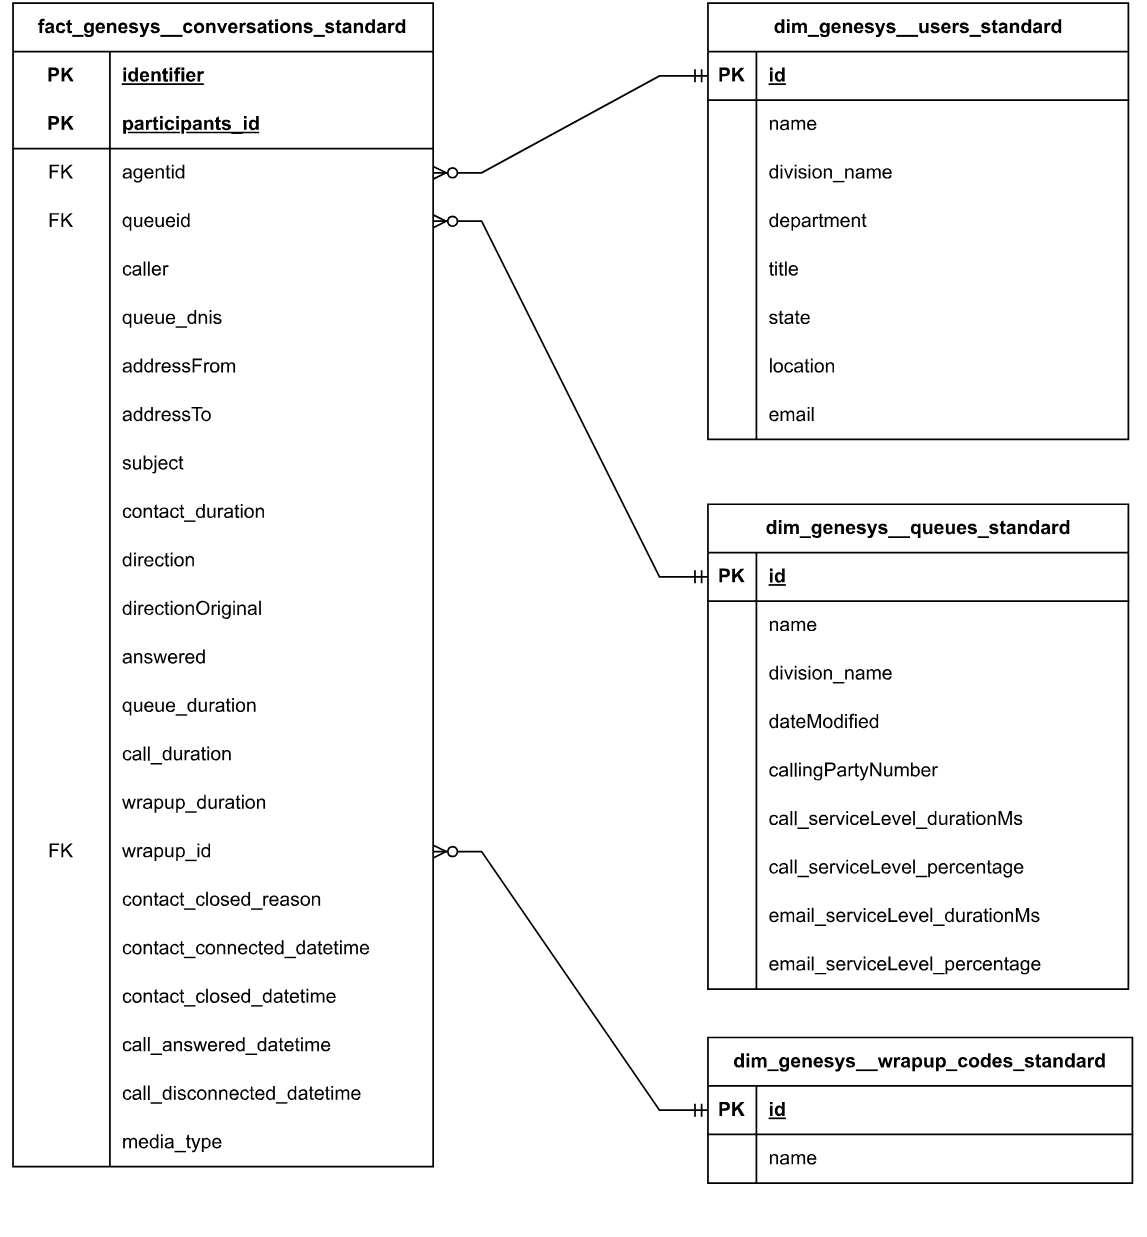
\includegraphics[width=1\textwidth]{media/data_spec.png}
    \caption{Käytettävän datan rakenne. Keskustelutiedot ovat päätaulussa, ja niihin liittyviä tietoja voidaan hakea liittyvistä tauluista.}
    \label{fig:data_spec}
  \end{center}
\end{figure}
\begin{appendices}
  \section{Linear Algebra}
  blbalbal

  \section{Probability theory}
  blbalbak

  \section{Full semantic view}
  \begin{lstlisting}[language=yaml]
name: SEM_VERBOSE
description: |-
  Semantic model that models conversations data from Genesys Cloud contact center software.
  This semantic model is more verbose and detailed than sem_conv_minimal and is designed to
  be used when the user wants to have more detailed information about conversations, queues, agents and
  wrap-up codes. For a more minimalistic model with only the most essential metrics and dimensions,
  see sem_conv_minimal.
tables:
  - name: AGENTS
    description: |-
      Employees/Agents in Genesys that handle conversations. Agents are divided to teams that are
              shown by their division_name field. Agents can have different attributes such as department, title, etc.
    base_table:
      database: DEV
      schema: DBT_OM
      table: DIM_GENESYS__USERS_STANDARD
    dimensions:
      - name: A_DEPARTMENT
        description: |-
          The department of the agent. Departments corralate to physcial locations
                  Moment Digital has offices at.
        expr: agents.department
        data_type: VARCHAR(16777216)
      - name: A_DIVISION_NAME
        description: The division name of the agent. Can also be called team in some contexts.
        expr: agents.division_name
        data_type: VARCHAR(16777216)
      - name: A_EMAIL
        description: The email address of the agent
        expr: agents.email
        data_type: VARCHAR(16777216)
      - name: A_NAME
        description: The name of the agent
        expr: agents.name
        data_type: VARCHAR(16777216)
      - name: A_TITLE
        description: |-
          The title of the agent. Agents are tittled "Asiakasneuvoja" other titels are
                  experts or supervisors
        expr: agents.title
        data_type: VARCHAR(16777216)
    primary_key:
      columns:
        - ID
  - name: CALE
    description: Calendar table for date dimensions
    base_table:
      database: DEV
      schema: DBT_OM
      table: DIM_CALENDAR
    dimensions:
      - name: CAL_DATE_DAY
        description: The date of the contact connected
        expr: cale.date_day
        data_type: DATE
      - name: CAL_DAY_OF_MONTH
        description: Day of the month (1-31)
        expr: cale.day_of_month
        data_type: NUMBER(2,0)
      - name: CAL_DAY_OF_WEEK_NAME
        description: The name of the day of the week (e.g., Monday, Tuesday)
        expr: cale.day_of_week_name
        data_type: VARCHAR(134217728)
      - name: CAL_MONTH_NAME
        description: Full name of the month (e.g., January, February)
        expr: cale.month_name
        data_type: VARCHAR(134217728)
      - name: CAL_MONTH_OF_YEAR
        description: Month number of the year (1-12)
        expr: cale.month_of_year
        data_type: NUMBER(38,0)
      - name: CAL_QUARTER_OF_YEAR
        description: Quarter number of the year (1-4)
        expr: cale.quarter_of_year
        data_type: NUMBER(38,0)
      - name: CAL_WEEK_OF_YEAR
        description: Week number of the year
        expr: cale.week_of_year
        data_type: NUMBER(38,0)
      - name: CAL_YEAR_NUMBER
        description: The year number
        expr: cale.year_number
        data_type: NUMBER(38,0)
    primary_key:
      columns:
        - DATE_DAY
  - name: CONV
    description: |-
      All Genesys conversations. Includes one record per agent participant per conversation,
              so conversations with multiple agent participants will have multiple records. Conversation
              can be a call, a callback, an email or message depending on the media type. And they have
              initial direction (inbound or outbound) and a current direction which can change over
              the course of the conversation.
    base_table:
      database: DEV
      schema: DBT_OM
      table: FACT_GENESYS__CONVERSATIONS_STANDARD
    dimensions:
      - name: C_ADDRESS_FROM
        description: Source address for the interaction. Only present in email contacts..
        expr: conv.address_from
        data_type: VARCHAR(16777216)
      - name: C_ADDRESS_TO
        description: Destination address for the interaction. Only present in email contacts..
        expr: conv.address_to
        data_type: VARCHAR(16777216)
      - name: C_ANSWERED
        description: |-
          Whether the contact was answered or whether the customer answered the call
                  in case of outbound calls. 1 if answered, 0 if not answered.
        expr: conv.answered
        data_type: NUMBER(38,0)
      - name: C_CALL_ANSWERED_DATETIME
        description: The datetime when the contact was answered. Null if the contact was not answered
        expr: conv.call_answered_datetime
        data_type: TIMESTAMP_NTZ(9)
      - name: C_CALL_DISCONNECTED_DATETIME
        description: The datetime when the contact was disconnected. Null if the contact was not answered
        expr: conv.call_disconnected_datetime
        data_type: TIMESTAMP_NTZ(9)
      - name: C_CALLER
        description: |-
          Originating caller address/ANI for the interaction.
                  Only present for phone interactions this is the caller phone number
        expr: conv.callers
        data_type: VARCHAR(16777216)
      - name: C_CONTACT_CLOSED_DATETIME
        description: The datetime when the contact was closed
        expr: conv.contact_closed_datetime
        data_type: TIMESTAMP_NTZ(9)
      - name: C_CONTACT_CLOSED_REASON
        description: |-
          The reason the interaction was closed. Most relevant are "client" which means the agent
                  closed the interaction and "peer" which means the customer closed the interaction.
        expr: conv.contact_closed_reason
        data_type: VARCHAR(16777216)
      - name: C_CONTACT_CONNECTED_DATETIME
        description: The datetime when the contact was connected
        expr: conv.contact_connected_datetime
        data_type: TIMESTAMP_NTZ(9)
      - name: C_DIRECTION
        description: |-
          The current direction of the conversation, either inbound or outbound. Usually both
                  current and original direction are the same, but in callbacks the original direction is inbound
                  and current direction is outbound.
        expr: conv.direction
        data_type: VARCHAR(16777216)
      - name: C_DIRECTION_ORIGINAL
        description: |-
          The original direction of the conversation, either inbound or outbound. By default most
                  metrics should be calculated using only originally inbound contacts, unless otherwise specified.
        expr: conv.direction_original
        data_type: VARCHAR(16777216)
      - name: C_MEDIA_TYPE
        description: |-
          The type of media. Ether call, callback, email, voice or message. Call is legacy
                  type that can include both calls and callbacks, but callbacks can be identified by their direction fields.
                  Voice is the current media type for calls that are not callbacks.
        expr: conv.media_type
        data_type: VARCHAR(16777216)
      - name: C_SUBJECT
        description: The subject of the conversation. Only present in email contacts.
        expr: conv.subject
        data_type: VARCHAR(16777216)
      - name: C_WRAPUPID
        description: Wrap-up code identifier applied to the interaction (if any).
        expr: conv.wrapupid
        data_type: VARCHAR(16777216)
    facts:
      - name: CALL_DURATION
        description: Duration of the actual call in seconds. The time the customer speaks to an agent
        expr: conv.call_duration
        data_type: NUMBER(38,0)
        access_modifier: public_access
      - name: CONTACT_DURATION
        description: Total duration of the contact in seconds. call_duration + wrapup_duration
        expr: conv.contact_duration
        data_type: NUMBER(38,0)
        access_modifier: public_access
      - name: QUEUE_DURATION
        description: Duration the contact spent in queue in seconds
        expr: conv.queue_duration
        data_type: NUMBER(38,0)
        access_modifier: public_access
      - name: WRAPUP_DURATION
        description: |-
          Duration of the wrap-up time in seconds. Duration of the after call work.
                  Should not be included when calculating email durations
        expr: conv.wrapup_duration
        data_type: NUMBER(38,0)
        access_modifier: public_access
    metrics:
      - name: ANSWER_PERCENTAGE
        description: |-
          Ratio of answered contacts to total inbound contacts, excluding short-abandons (default X=0).
                  Often queried only for calls
                  in that case the media type should be filtered to include only call and voice and current
                  direction should be also inbound.
        expr: |-
          conv.answered_contacts /
                  nullif(
                  (
                      conv.inbound_contacts -
                      sum(case when conv.queue_duration <= 0
                                    and conv.answered = 0
                                    and conv.direction_original = 'inbound'
                               then 1 else 0 end)
                  ),0)
        access_modifier: public_access
      - name: ANSWERED_CONTACTS
        description: |-
          Total number of answered inbound contacts. Often queried only for calls
                  in that case the media type should be filtered to include only call and voice and current
                  direction should be also inbound.
        expr: |-
          count(distinct case when conv.answered = 1
                                           and conv.direction_original = 'inbound'
                                      then conv.identifier end)
        access_modifier: public_access
      - name: ANSWERED_CONTACTS_UNIQUE
        description: Total number of unique answered inbound callers
        expr: |-
          count(distinct case when conv.answered = 1
                                           and conv.direction_original = 'inbound'
                                      then conv.c_caller end)
        access_modifier: public_access
      - name: AVERAGE_CALL_DURATION
        description: Average call duration in seconds
        expr: sum(conv.call_duration)
        access_modifier: public_access
      - name: AVERAGE_QUEUE_DURATION
        description: Average queue duration in seconds
        expr: avg(conv.queue_duration)
        access_modifier: public_access
      - name: AVERAGE_WRAPUP_DURATION
        description: Average wrap-up duration in seconds
        expr: sum(conv.wrapup_duration)
        access_modifier: public_access
      - name: INBOUND_CONTACTS
        description: |-
          Total number of inbound contacts. Often queried only for calls
                  in that case the media type should be filtered to include only call, callbacks and voice.
        expr: |-
          count(distinct case when conv.direction_original = 'inbound'
                                      then conv.identifier end)
        access_modifier: public_access
      - name: REJECT_PERCENTAGE
        description: Ratio of rejected contacts to total inbound contacts, including short-abandons
        expr: conv.rejected_contacts / nullif(conv.inbound_contacts, 0)
        access_modifier: public_access
      - name: REJECTED_CONTACTS
        description: Total number of rejected inbound contacts, including short-abandons
        expr: |-
          count(distinct case when conv.answered = 0
                      and conv.direction_original = 'inbound' then conv.identifier end)
        access_modifier: public_access
      - name: REJECTED_INCOMING_UNIQUE
        description: Total number of rejected inbound contacts
        expr: conv.total_incoming_unique - conv.answered_contacts_unique
        access_modifier: public_access
      - name: SERVICE_LEVEL_PERCENTAGE
        description: |-
          Service level percentage: ratio of inbound contacts answered within service
                  level target to total eligible inbound contacts. Includes only inbound calls. Never callbacks
                  or emails or outbound contacts.
        expr: |-
          count(distinct case when conv.queue_duration <= queu.q_call_service_level_duration_seconds
                                           and conv.answered = 1
                                           and conv.c_direction = 'inbound'
                                           and conv.c_media_type in ('call', 'voice')
                                      then conv.identifier end)
                  /
                  nullif(
                  (
                      count(distinct case when conv.c_direction = 'inbound'
                                               and conv.answered = 1
                                          then conv.identifier end)
                      + count(distinct case when conv.queue_duration > queu.q_call_service_level_duration_seconds
                                                 and conv.answered = 0
                                                 and conv.c_direction = 'inbound'
                                                 and conv.c_media_type in ('call', 'voice')
                                            then conv.identifier end)
                  ),0)
        access_modifier: public_access
      - name: TOTAL_CALL_DURATION
        description: Total call duration in seconds
        expr: sum(conv.call_duration)
        access_modifier: public_access
      - name: TOTAL_CONTACT_DURATION
        description: Total contact duration in seconds
        expr: sum(conv.contact_duration)
        access_modifier: public_access
      - name: TOTAL_CONTACTS
        description: Total number of contacts
        expr: count(*)
        access_modifier: public_access
      - name: TOTAL_INCOMING_UNIQUE
        description: Total number of unique incoming contacts
        expr: count(distinct case when conv.direction_original = 'inbound' then conv.callers end)
        access_modifier: public_access
      - name: TOTAL_QUEUE_DURATION
        description: Total queue duration in seconds
        expr: sum(conv.queue_duration)
        access_modifier: public_access
      - name: TOTAL_WRAPUP_DURATION
        description: Total wrap-up duration in seconds
        expr: sum(conv.wrapup_duration)
        access_modifier: public_access
    primary_key:
      columns:
        - PARTICIPANTS_ID
        - IDENTIFIER
  - name: QUEU
    description: |-
      All Genesys queues. One service can have multiple queues.
              This is usually evident by similarities in queue names.
    base_table:
      database: DEV
      schema: DBT_OM
      table: DIM_GENESYS__QUEUES_STANDARD
    dimensions:
      - name: Q_CALL_SERVICE_LEVEL_DURATION_SECONDS
        description: Call service level target duration in seconds
        expr: queu.call_service_level_duration_seconds
        data_type: NUMBER(38,6)
      - name: Q_CALL_SERVICE_LEVEL_PERCENTAGE
        description: Call service level target percentage
        expr: queu.call_service_level_percentage
        data_type: NUMBER(38,0)
      - name: Q_DIVISION_NAME
        description: |-
          Division name associated with the queue. These are loosely correlated with agents
                  teams, but not always. This is because some services require their own division for technical reasons.
        expr: queu.division_name
        data_type: VARCHAR(16777216)
      - name: Q_EMAIL_SERVICE_LEVEL_DURATION_SECONDS
        description: Email service level target duration in seconds
        expr: queu.email_service_level_duration_seconds
        data_type: NUMBER(38,6)
      - name: Q_EMAIL_SERVICE_LEVEL_PERCENTAGE
        description: Email service level target percentage
        expr: queu.email_service_level_percentage
        data_type: NUMBER(38,0)
      - name: Q_NAME
        description: The name of the queue
        expr: queu.name
        data_type: VARCHAR(16777216)
    primary_key:
      columns:
        - ID
  - name: WRAP
    description: |-
      Wrap up codes. Wrap up codes are not used in every queue/service,
              but when they are used they are applied to conversations after they are finished to
              categorize the reason for the contact or any other relevant categorization.
              Not all conversations will have wrap up codes, but when they do they can be used
              for filtering and analysis.
    base_table:
      database: DEV
      schema: DBT_OM
      table: DIM_GENESYS__WRAPUP_CODES_STANDARD
    dimensions:
      - name: W_NAME
        description: The name of the wrap-up code
        expr: wrap.name
        data_type: VARCHAR(16777216)
    primary_key:
      columns:
        - ID
relationships:
  - name: CONVERSATIONS_CONNECTED_TO_CALENDAR
    left_table: CONV
    right_table: CALE
    relationship_columns:
      - left_column: CONTACT_CONNECTED_DATE
        right_column: DATE_DAY
  - name: CONVERSATIONS_TO_AGENTS
    left_table: CONV
    right_table: AGENTS
    relationship_columns:
      - left_column: AGENTID
        right_column: ID
  - name: CONVERSATIONS_TO_QUEUES
    left_table: CONV
    right_table: QUEU
    relationship_columns:
      - left_column: QUEUEID
        right_column: ID
  - name: CONVERSATIONS_TO_WRAPUP
    left_table: CONV
    right_table: WRAP
    relationship_columns:
      - left_column: WRAPUPID
        right_column: ID
\end{lstlisting}

\end{appendices}
\begin{thebibliography}{99}
  \bibitem{NewtLeib} Newton ja Leibniz
  \bibitem{Riemann} Riemann
  \bibitem{CortexAnalyst} Snowflake Inc. (n.d.). Cortex Analyst. Retrieved April 22, 2026, from \href{https://docs.snowflake.com/en/user-guide/snowflake-cortex/cortex-analyst}{https://docs.snowflake.com/en/user-guide/snowflake-cortex/cortex-analyst}
\end{thebibliography}
\end{document}
